\documentclass[10pt,svgnames,usenames,table]{beamer} %,handout si version papier
\NeedsTeXFormat{LaTeX2e}

\usepackage[T1]{fontenc}
%\usepackage[utf8x]{inputenc}
\usepackage[french]{babel}
\usepackage{lmodern}
\usepackage{amsmath,amsthm,amssymb}        % un packages mathématiques
\usepackage{pifont}
\newcommand{\cmark}{\ding{51}}%
\newcommand{\xmark}{\ding{55}}%
\usepackage{xcolor}         % pour définir plus de couleurs
\usepackage{graphicx}       % pour insérer des figures
\usepackage{lmodern}
\usepackage{url}
\urlstyle{sf}
\usepackage{lastpage}
\usepackage{endnotes}
\usepackage{listings}
%\usepackage{listingsutf8}

\usepackage{siunitx}
\usepackage{circuitikz}
\usepackage{chemfig}
\usepackage[version=3]{mhchem}

\usepackage[french]{varioref}
\usepackage{wrapfig}
\usepackage{pdfpages}
\usepackage{verbatim}
\usepackage{graphicx}

\usepackage{xspace}
\usepackage{mdframed}
\usepackage{pgfplots}
\usepackage[french]{varioref} % \vpageref
\usepackage{epstopdf}
\usepackage{pdflscape} %% portrait


\newcommand{\badet}{et}
\newcommand{\goodet}{\mathbin{\mathrm{et}}}

\DeclareMathOperator{\sumN}{\sum_{i=1}^n}
\DeclareMathOperator{\var}{\mathrm{Var}}


\usetheme[compress]{Singapore} % theme
\usefonttheme[onlymath]{serif} % to see the difference when I do mathsf
%\renewcommand\sfdefault{cmss} % Polices


\definecolor{gris}{RGB}{228,228,228}
\definecolor{bleu}{RGB}{34,148,255}
\definecolor{darkgray}{rgb}{0.3,0.3,0.3}
\definecolor{codeGreen}{rgb}{0,0.5,0}
\lstset{
      language=TeX,
      flexiblecolumns=true,
      numbers=left,
      stepnumber=1,
      numberstyle=\ttfamily\tiny,
      keywordstyle=\ttfamily\textcolor{blue},
      stringstyle=\ttfamily\textcolor{red},
      commentstyle=\ttfamily\textcolor{codeGreen},
      breaklines=true,
      extendedchars=true,
      basicstyle=\ttfamily\scriptsize,
      showstringspaces=false,
      morekeywords={usepackage,documentclass,begin,textbf,textit,texttt,ref,includegraphics,caption,label,setlength,mathbb,notag,frac,num,si,ang,SI,textwidth,percent,meter,ohm,joule,second,more,section,subsection,tableofcontents,setstretch,TeX,LaTeX,sffamily,emph,chemfig,pageref,vpageref,date,maketitle,institute,author,and,textsc,title,includeonly,include,clearpage,newcommand,mathsf,renewcommand,per,celsius,square,volt,cubic,lumen,farad,DeclareMathOperator,mathrm,mathcal,captionof,lstinputlisting,lstinline,tiny,small,normalsize,large,Large,huge,Huge},
      frame=single,
      extendedchars=true,
      inputencoding=utf8x,
	    literate={á}{{\'a}}1 {ã}{{\~a}}1 {é}{{\'e}}1 {è}{{\`e}}1 {à}{{\`a }}1
    }
%\lstset{inputencoding=utf8/latin1}
\lstset{literate=
{á}{{\'a}}1
{à}{{\`a}}1
{À}{{\`A}}1
{ã}{{\~a}}1
{é}{{\'e}}1
{è}{{\`e}}1
{ê}{{\^e}}1
{î}{{\^i}}1
{í}{{\'i}}1
{ó}{{\'o}}1
{õ}{{\~o}}1
{ô}{{\^o}}1
{ú}{{\'u}}1
{ü}{{\"u}}1
{ç}{{\c{c}}}1
}
\lstset{keepspaces}
\lstdefinestyle{nonumbers}
{numbers=none}


% Pour personnaliser la barre de navigation du dessous
\setbeamertemplate{navigation symbols}{
	%\insertslidenavigationsymbol
	%\insertframenavigationsymbol
	%\insertsubsectionnavigationsymbol
	\quad\textbf{\insertframenumber/\inserttotalframenumber} % Numéro de page
	%\insertsectionnavigationsymbol
	%\insertdocnavigationsymbol
	%\insertbackfindforwardnavigationsymbol
}
% Supprimer les icones de navigation (pour les transparents)
%\setbeamertemplate{navigation symbols}{}

% Mettre les icones de navigation en mode vertical (pour projection)
% \setbeamertemplate{navigation symbols}[vertical]

\setbeamercolor{section in head/foot}{use=structure,bg=structure.fg!25!bg} % "Amélioration du jeu de couleur"
%\useoutertheme[subsection=true]{smoothbars} % Pour avoir un rappel de la subsection
\setbeamerfont{frametitle}{series=\bfseries}
\setbeamertemplate{frametitle}[default][center] % Titre centré et bien placé.

% Comportement des itemize
\setbeamertemplate{itemize item}[ball]
\setbeamertemplate{itemize subitem}[triangle]
\setbeamertemplate{itemize subsubitem}[circle]

% "Fioriture de style" : qd <x-> dans les item, les autres en gris clair
\beamertemplatetransparentcovered

% Les block arrondis et ombrés dans la couleur que je veux
\setbeamertemplate{blocks}[rounded][shadow=true]
\definecolor{normalBlockColor}{RGB}{255,255,255}
\definecolor{normalTitleBlockColor}{RGB}{0,0,102}
\definecolor{normalBlockTextColor}{RGB}{0,0,0}
\definecolor{normalBlockTitleTextColor}{RGB}{255,255,255}
\definecolor{exampleBlockColor}{RGB}{202,251,197}
\definecolor{exampleTitleBlockColor}{RGB}{166,241,158}
\definecolor{exampleBlockTextColor}{RGB}{0,0,0}
\definecolor{exampleBlockTitleTextColor}{RGB}{0,120,0}
\definecolor{alertBlockColor}{RGB}{248,218,218}
\definecolor{alertTitleBlockColor}{RGB}{244,108,108}
\definecolor{alertBlockTextColor}{RGB}{0,0,0}
\definecolor{alertBlockTitleTextColor}{RGB}{120,0,0}
\setbeamercolor*{block title}{fg=normalBlockTitleTextColor,bg=normalTitleBlockColor}
\setbeamercolor*{block body}{fg=normalBlockTextColor,bg=normalBlockColor}
\setbeamercolor*{block title alerted}{fg=alertBlockTitleTextColor,bg=alertTitleBlockColor}
\setbeamercolor*{block body alerted}{fg=alertBlockTextColor,bg=alertBlockColor}
\setbeamercolor*{block title example}{fg=exampleBlockTitleTextColor,bg=exampleTitleBlockColor}
\setbeamercolor*{block body example}{fg=exampleBlockTextColor,bg=exampleBlockColor}
\setbeamerfont{block title}{size={}}

% Pour rendre les toc plus compactes (pour éviter que ça déborde)
\makeatletter
\patchcmd{\beamer@sectionintoc}{\vskip1.5em}{\vskip0.5em}{}{}
\makeatother
\setbeamerfont{subsection in toc}{size=\scriptsize}


\graphicspath{{img/}}


\newcommand{\badet}{et}
\newcommand{\goodet}{\mathbin{\mathrm{et}}}
\DeclareMathOperator{\sumN}{\sum_{i=1}^n}
\DeclareMathOperator{\var}{\mathrm{Var}}


\graphicspath{{img/}}
\definecolor{gris}{RGB}{228,228,228}
\definecolor{bleu}{RGB}{34,148,255}
\definecolor{darkgray}{rgb}{0.3,0.3,0.3}
\usefonttheme[onlymath]{serif} % to see the difference when I do mathsf


\logo{
\includegraphics[height=5mm]{logo.pdf}}
\institute{Louvain-li-Nux}
\title{\textbf{Formation \LaTeX}\\
Introduction à l'écriture de documents avec \LaTeX}
\author{Morgan \textsc{Leclerc} \and Martin \textsc{Vandenbussche}}

\date{04 décembre 2019}

% A changer (selon Arnaud) le utf8x pas aligné slide 12/30
% maketitle
%
%
\begin{document}

%\begin{frame}
%  \begin{center}\Large
%  Suivez cette présentation sur votre ordinateur :-)
%
%  \vspace{1cm}
%  \end{center}
%\end{frame}


\begin{frame}
  \maketitle
%  Merci à Jolan \textsc{Wolter}, Thomas \textsc{Vanzieleghem}, David \textsc{Ernst}, Matthieu \textsc{Baerts}, Arnaud \textsc{Cerckel}, Benoît \textsc{Legat}, Mattéo \textsc{Couplet}, Geoffroy \textsc{Jacquet}, Xavier \textsc{Lambein}, Sébastien \textsc{de Longueville} et Gaëtan \textsc{Cassiers} pour la réalisation des précédentes versions de ces transparents

\end{frame}

\AtBeginSection[]
  {
     \begin{frame}<beamer>
     \frametitle{\insertsection}
     \tableofcontents[hideothersubsections]
     \end{frame}
  }

\section{Introduction}
\subsection{Qu'est-ce que \LaTeX{}?}
\begin{frame}
\frametitle{Qu'est-ce que \LaTeX}

\begin{itemize}
\item \LaTeX{} $=$ méthode privilégiée d'écriture de documents scientifiques
 \vspace{0.5cm}
\item \LaTeX{} $ \neq$ WYSIWYG (What You See Is What You Get)
\end{itemize}

\end{frame}

\subsection{Pourquoi \LaTeX{}?}
\begin{frame}{Pourquoi \LaTeX{}?}

  \begin{itemize}
      \item Documents de qualité professionnelle
    \item Facilité d'emploi des :
    \begin{itemize}
        \item formules mathématiques
        \item tables des matières
        \item images et tableaux
        \item références bibliographiques
        \item références croisées
        \item \ldots{}
    \end{itemize}
    \item Gratuit
    \item Stable, même pour les très gros documents
  \end{itemize}
\end{frame}

\begin{frame}{Pourquoi \LaTeX{}?}

\begin{figure}[htbp]
\begin{center}
\includegraphics[height=6.5cm]{latex_exemples}
\end{center}
\end{figure}
\end{frame}

%-----------------------
\subsection{Pourquoi pas \LaTeX{}?}
\begin{frame}{Pourquoi pas \LaTeX{}?}

  \begin{itemize}
    \item Prise en main plus longue que pour traitement de texte WYSIWYG
    \item Je suis allergique à toute forme de code informatique
    \item J'ai des actions Microsoft
    \item Je ne trouve pas le ``\textbackslash'' sur mon clavier
  \end{itemize}
\end{frame}

\begin{comment}
\begin{frame}{Oui mais\ldots{}}
  \begin{center}
    %\resizebox{\textwidth}{!}{
    \begin{tikzpicture}
      \begin{axis}[xmin=0, xmax=4, ymin=-2, ymax=5, ticks=none,
          xlabel={Expérience}, ylabel=Productivité,
        legend style={at={(0.01,0.99)}, anchor=north west}]
        \addplot[smooth, color=blue]{x-0.05};
        \addlegendentry{\LaTeX}
        \addplot[smooth, color=red,domain=0:5]{sqrt(x)};
        \addlegendentry{Word}
        %\xlabel{Productivité}
        %\ylabel{Expérience/maitrise}
      \end{axis}
      \foreach \x/\com/\deltax/\deltay/\adj in {
        %\small
        {1.1}/{\scriptsize Maintenant}/{0}/{0.8}/below,
        {2.2}/{\scriptsize Après la formation}/{0}/{0.4}/below,
        %{4.6}/{À l'heure de votre mémoire}/{0}/{1.2}/below
        {4.6}/{\scriptsize Au bout de quelques semaines}/{0}/{1.2}/below
      } {
        %\fill \coord circle (100pt) node[\adj] {$\coord$};
        \draw[dashed] (\x,0) -- (\x+\deltax,\deltay) node[above] {\com};
        %\draw (\x+\deltax,\deltay) node {\com};
      }
    \end{tikzpicture}
    %}
  \end{center}
\end{frame}
\end{comment}
%-----------------------
\subsection{Les Outils}
\begin{frame}{Quels logiciels pour utiliser \LaTeX{}?}

  \begin{itemize}
      \item GNU/Linux
      \begin{itemize}
          \item Distribution \LaTeX{} : \textbf{TeXLive}
          {\tiny (\lstinline|sudo apt install texlive-full|)}
        \item Éditeur : \textbf{\href{http://www.xm1math.net/texmaker/}{TeXMaker}}
      \end{itemize}
      \item Windows
      \begin{itemize}
        \item Distribution \LaTeX{} : \textbf{TeXLive}
        \item Éditeur : \textbf{\href{http://www.xm1math.net/texmaker/}{TeXMaker}}
      \end{itemize}
      \item Mac OS
      \begin{itemize}
        \item Distribution \LaTeX{} : \textbf{\href{https://www.tug.org/mactex/}{MacTeX}}
        \item Éditeur : \textbf{\href{http://www.xm1math.net/texmaker/}{TeXMaker}}
      \end{itemize}
      \item Dans votre navigateur
      \begin{itemize}
        \item \textbf{\url{www.overleaf.com}}
      \end{itemize}
  \end{itemize}
  Pour cet atelier, nous vous conseillons d'utiliser \textbf{overleaf} sur votre propre PC.
\end{frame}

\subsection{Symboles spéciaux sur Mac}
\begin{frame}{Symboles spéciaux sur Mac}
  \begin{center}
    \begin{tabular}{|lc|l|}
      \hline
      Symbole & & Raccourci clavier \\\hline
      \textit{backslash} & \textbackslash & alt + shift + / \\
      accolade & \{\} & alt + () \\
      crochet & $[]$ & alt + shift + () \\
      \textit{pipe} & | & alt + shift + L \\
      \hline
    \end{tabular}
  \end{center}
\end{frame}

\section{Les concepts de base}
\subsection{Les fichiers}

\begin{frame}{Les fichiers}

    \begin{center}
        \includegraphics[height=3cm]{compilation.jpg}
    \end{center}

    \begin{itemize}
        \item Fichier source = essais\alert{\textbf{.tex}}
        \item Fichier de bibliographie = essais\alert{\textbf{.bib}}
        \item Lors de compilation $\rightarrow$ création de nombreux fichiers annexes
        \begin{itemize}
            \item style, class;
            \item structure du document;
            \item table des matières, liste des figures;
            \item liste des références;
            \item \ldots{}
        \end{itemize}
        \item Création d'un fichier essais\alert{\textbf{.pdf}}
    \end{itemize}
\end{frame}

%-----------------------
\subsection{La structure du fichier}

\begin{frame}[fragile,label=frame:structure]{Structure générale du document I}
\framesubtitle{Document minimal}
\small

\begin{lstlisting}[style=nonumbers]
\documentclass{article} %Type de document

%Préambule
%On charge ici les packages

\begin{document}
    %Corps du document
\end{document}
\end{lstlisting}
\begin{itemize}
    \item On charge les \textit{packages} et effectue certains réglages dans le préambule.
    \item On écrit le contenu de son document entre \lstinline|\begin{document}| et \lstinline|\end{document}|.
    \item Commentaires introduits par \%
\end{itemize}

\end{frame}

\begin{frame}[fragile]{Structure générale du document II}
\framesubtitle{Exemple de document type}
\small
\begin{tabular}{ll}
  Type de document &
  \lstinline|\documentclass[a4paper, 10pt]{scrartcl}|\\
  Utilisation de \textit{package} &
  \lstinline|\usepackage[utf8]{inputenc}|\\
  Utilisation de \textit{package} &
  \lstinline|\usepackage[T1]{fontenc}|\\
  Utilisation de \textit{package} &
  \lstinline|\usepackage[french]{babel}|\\
   &\\
  Début du document &
  \lstinline|\begin{document}|\\
  Corps du document &
  \lstinline|Ceci est mon premier document en Latex !!!|\\
  Fin du document &
  \lstinline|\end{document}|\\
\end{tabular}
\end{frame}

\subsection{Commandes et environnements}
\begin{frame}[fragile]{Les Commandes}
\begin{itemize}
\item \textbf{Commande}
    \begin{itemize}
    \item Débute par \textbackslash
    \item Peut prendre plusieurs arguements, placés entre accolades
    \item Permet d'insérer des symboles
    \end{itemize}
    \begin{lstlisting}[style=nonumbers]
\commandName[options]{FirstParameter} ... {LastParameter}
    \end{lstlisting}
    \begin{center}
    \begin{tabular}{lllll}
    \lstinline|\implies| & $\implies$ & & \lstinline|\textbf{texte}| & \textbf{texte}
    \end{tabular}
    \end{center}
\end{itemize}
\end{frame}

\begin{frame}[fragile]{Les Environnements}
\begin{itemize}
\item \textbf{Environnement}
    \begin{itemize}
    \item S'applique à des \textit{portions de texte} et permet par exemple d'appliquer une règle de mise en page
    \item Délimité par \lstinline|\begin{}| et \lstinline|\end{}|
    \end{itemize}
    \begin{lstlisting}[style=nonumbers]
\begin{EnvironnementName}[options]

\end{EnvironnementName}
    \end{lstlisting}
    \begin{center}
      \begin{columns}
      \begin{column}{0.5\textwidth}
      \begin{lstlisting}[style=nonumbers]
\begin{figure}
    \centering
    
\includegraphics{logo-uclouvain.eps}
    \caption{Voici le logo UCLouvain}
    \label{fig:ucl}
\end{figure}
      \end{lstlisting}
      \end{column}
      \begin{column}{0.5\textwidth}
      \begin{figure}[!ht]
          \centering
          
\includegraphics[width=0.50\textwidth]{logo-uclouvain.pdf}
          \caption{Voici le logo UCLouvain}
          \label{fig:ucl}
      \end{figure}
      \end{column}
      \end{columns}
    \end{center}
\end{itemize}
\end{frame}
%-----------------------

\subsection{Les classes}

\begin{frame}[fragile]{Les principales classes de document}
\begin{tabular}{p{0.2\textwidth}p{0.8\textwidth}}
  \textbf{scrartcl} & pour les articles de journaux scientifiques, présentations, rapports courts,\dots \\ \\
  \textbf{scrreprt} & pour de plus long rapports de plusieurs chapitres, petits livres, thèses,\dots \\ \\
  \textbf{beamer} & pour écrire des présentations (comme celle-ci) \\ \\
  \textbf{et beaucoup d'autres} & dont les références sont facilement trouvables sur Internet
\end{tabular}
%\vspace{1cm}
\begin{center}
\verb|\documentclass[a4paper,10pt]{|\alert{\texttt{scrartcl}}\verb|}|\\
\end{center}
\end{frame}

\subsection{Les options}

\begin{frame}[fragile]{Les principales options de document}
\begin{tabular}{lp{8cm}}
  \textbf{10pt, 11pt, 12pt} & pour la taille de police.\\
  \textbf{a4paper, a5paper} & pour la taille de page.\\
  \textbf{twoside} & pour des marges de livre
\end{tabular}
\vspace{1cm}
\begin{center}
\verb|\documentclass[|\alert{\texttt{a4paper,10pt}}\verb|]{scrartcl}|\\
\end{center}
\end{frame}

\subsection{Les packages}

\begin{frame}[fragile]{Les packages}
\begin{itemize}
\item Les \textbf{packages} sont des extensions contenant de nouveaux environnements et commandes
\item Appel du package dans le \textit{préambule} à l'aide de la commande \lstinline|\usepackage[options]{packageName}|
\end{itemize}
\vskip2em
\begin{tabular}{ll}
\lstinline|\usepackage[utf8]{inputenc}| & Utilisation des caractères accentués \\
\lstinline|\usepackage[T1]{fontenc}| & Permet d'utiliser tous les caractères du clavier \\
\lstinline|\usepackage[french]{babel}| & Spécifie la langue (français ici) \\
\lstinline|\usepackage{graphicx}| & Permet d'importer des images
\end{tabular}
\vskip2em
\begin{itemize}
    \item Les 3 premiers packages de l'exemple sont nécessaires à la compilation !
\end{itemize}
\end{frame}

\subsection{La structure du document}
\begin{frame}[fragile]{La structure logique du document}
    \begin{itemize}
        \item Structure logique du document uniquement
        \item \LaTeX{} se charge de la numérotation et de la mise en page\\
    \end{itemize}
    \vspace{1cm}

    \begin{itemize}
        \item \lstinline|\section{}|
        \item \lstinline|\subsection{}|
        \item \lstinline[mathescape]|\$\color{blue}{\texttt{paragraph}}${}| % Don't question it, it just works
    \end{itemize}

\end{frame}

\begin{frame}[fragile]{La structure logique du document}
\framesubtitle{Exemple}
    \begin{columns}
      \begin{column}{0.5\textwidth}
        \begin{lstlisting}[style=nonumbers,mathescape]
\section{Une $\color{black}{\texttt{section}}$}
\subsection{Une sous-$\color{black}{\texttt{section}}$}
\paragraph{Un paragraph} Le contenu de mon paragraphe sans alinéa.

Un paragraphe sans titre.
La première ligne a toujours un alinéa.

Un deuxième paragraphe sans titre.
À nouveau la première ligne a un alinéa.
        \end{lstlisting}
      \end{column}
      \begin{column}{0.5\textwidth}
        \fbox{
\includegraphics[width=1\textwidth,trim={1.5cm 14cm 1.5cm 1cm},clip]{examples/structure/build_latex/main.pdf}}
      \end{column}
    \end{columns}
    \begin{itemize}
    \item Pour créer un nouveau paragraphe, il suffit de faire deux retours à la ligne.
    \end{itemize}
\end{frame}

%-----------------------
\section{Mise en page générale}

\subsection{Titre}
\begin{frame}[fragile]{Titre}
    \begin{itemize}
        \item Informations données dans \lstinline|\author{}|, \lstinline|\date{}| and \lstinline|\title{}| \textbf{avant} le \lstinline|\begin{document}|
        \item Création de la page de titre avec \lstinline|\maketitle| \textbf{après} le \lstinline|\begin{document}|
    \end{itemize}
    \begin{columns}
      \begin{column}{0.5\textwidth}
        \begin{lstlisting}[style=nonumbers,mathescape]
\$\color{blue}{\texttt{subject}}${US Presidential Elections}
\title{FBI Investigations}
\$\color{blue}{\texttt{subtitle}}${Russian interference in the 2016 United States elections}

% Séparer les auteurs avec \and
\author{Donald Trump \and Vladimir Putin}

\date{}               % pas de date
\date{\$\color{blue}{\texttt{today}}$}         % aujourd'hui
\date{8 november 2016}

\begin{document}

\maketitle

\end{document}
        \end{lstlisting}
      \end{column}
      \begin{column}{0.5\textwidth}
    \centering
        \fbox{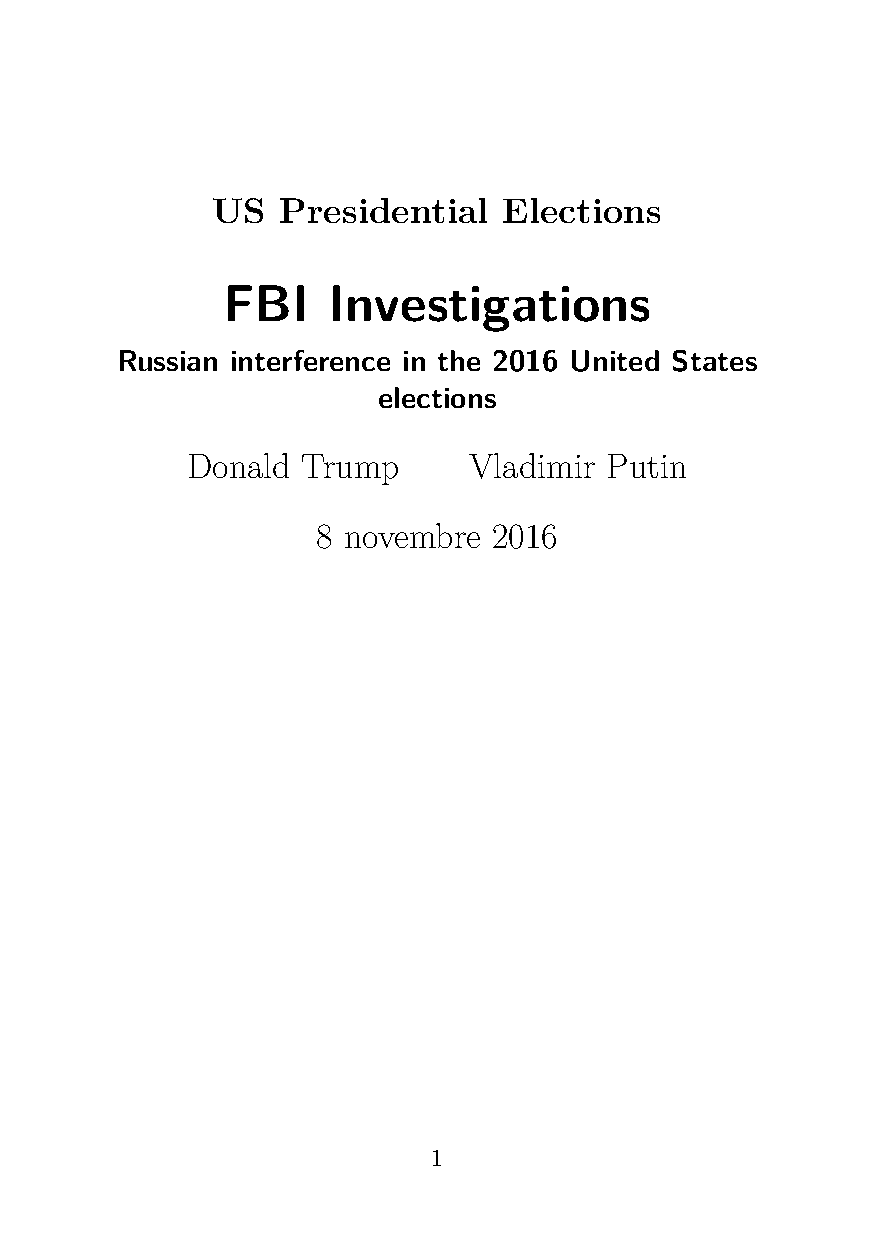
\includegraphics[width=1\textwidth,trim={1.5cm 10cm 1.5cm 1cm},clip]{examples/title/build_latex/main.pdf}}
      \end{column}
    \end{columns}
\end{frame}

\subsection{Le résumé ou abstract}
\begin{frame}[fragile]{Le résumé ou abstract}
    \begin{itemize}
        \item L'environnement \lstinline|abstract| permet de mettre en page un résumé au début du document.
    \end{itemize}
    \begin{columns}
      \begin{column}{0.5\textwidth}
        \begin{lstlisting}[style=nonumbers]
\begin{document}
...
\begin{abstract}
  Voici un résumé succint du contenu
  de mon document.
\end{abstract}
...
\end{document}
        \end{lstlisting}
      \end{column}
      \begin{column}{0.5\textwidth}
                \begin{abstract}
                    Voici un résumé succint du contenu de mon document.
                \end{abstract}
      \end{column}
    \end{columns}
\end{frame}

\subsection{La table des matières}
\begin{frame}[fragile]{Table des matières}
    \begin{itemize}
        \item La commande \lstinline|\tableofcontents| suffit pour générer toute la table des matières dynamiquement à partir desvos sections, sous-sections etc.
    \end{itemize}
    \begin{columns}
      \begin{column}{0.6\textwidth}
        \begin{lstlisting}[style=nonumbers]
\begin{document}

\tableofcontents % Table des matières

\section{Introduction}
Ceci est mon premier document en \TeX{}

\section{Le vif du sujet}
Le sujet est en or mais pas le vif.

\subsection{Mais quel est le sujet ?}
\LaTeX{}, ce logiciel d'exception !

\end{document}
        \end{lstlisting}
      \end{column}
      \begin{column}{0.4\textwidth}
        \begin{center}
          \fbox{\includegraphics[width=0.9\textwidth]{table.png}}
        \end{center}
      \end{column}
    \end{columns}
\end{frame}

%-----------------------
\subsection{Listes}
\begin{frame}[fragile]
  \frametitle{Listes}
  \begin{itemize}
    \item Pour faire des listes à puce, utiliser l'environnement \lstinline|itemize|.
    \begin{columns}
      \begin{column}{0.45\textwidth}
        \begin{lstlisting}[style=nonumbers]
\begin{itemize}
  \item Un chat;
  \item une poule;
  \item un chien.
\end{itemize}
        \end{lstlisting}
      \end{column}
      \begin{column}{0.45\textwidth}
        \begin{itemize}
          \item Un chat;
          \item une poule;
          \item un chien.
        \end{itemize}
      \end{column}
    \end{columns}

    \item Pour faire des listes numerotées, utiliser l'environnement \lstinline|enumerate|.
    \begin{columns}
      \begin{column}{0.45\textwidth}
        \begin{lstlisting}[style=nonumbers]
\begin{enumerate}
  \item Mettez de l'eau.
  \item Chauffer l'eau.
  \item Mettez les pasta.
\end{enumerate}
        \end{lstlisting}
      \end{column}
      \begin{column}{0.45\textwidth}
        \begin{enumerate}
          \item Mettez de l'eau.
          \item Chauffer l'eau.
          \item Mettez les pâtes.
        \end{enumerate}
      \end{column}
    \end{columns}
  \end{itemize}
\end{frame}

\subsection{Exercice 1}
\begin{frame}[fragile]{Premier exercice}
\begin{center}
\fbox{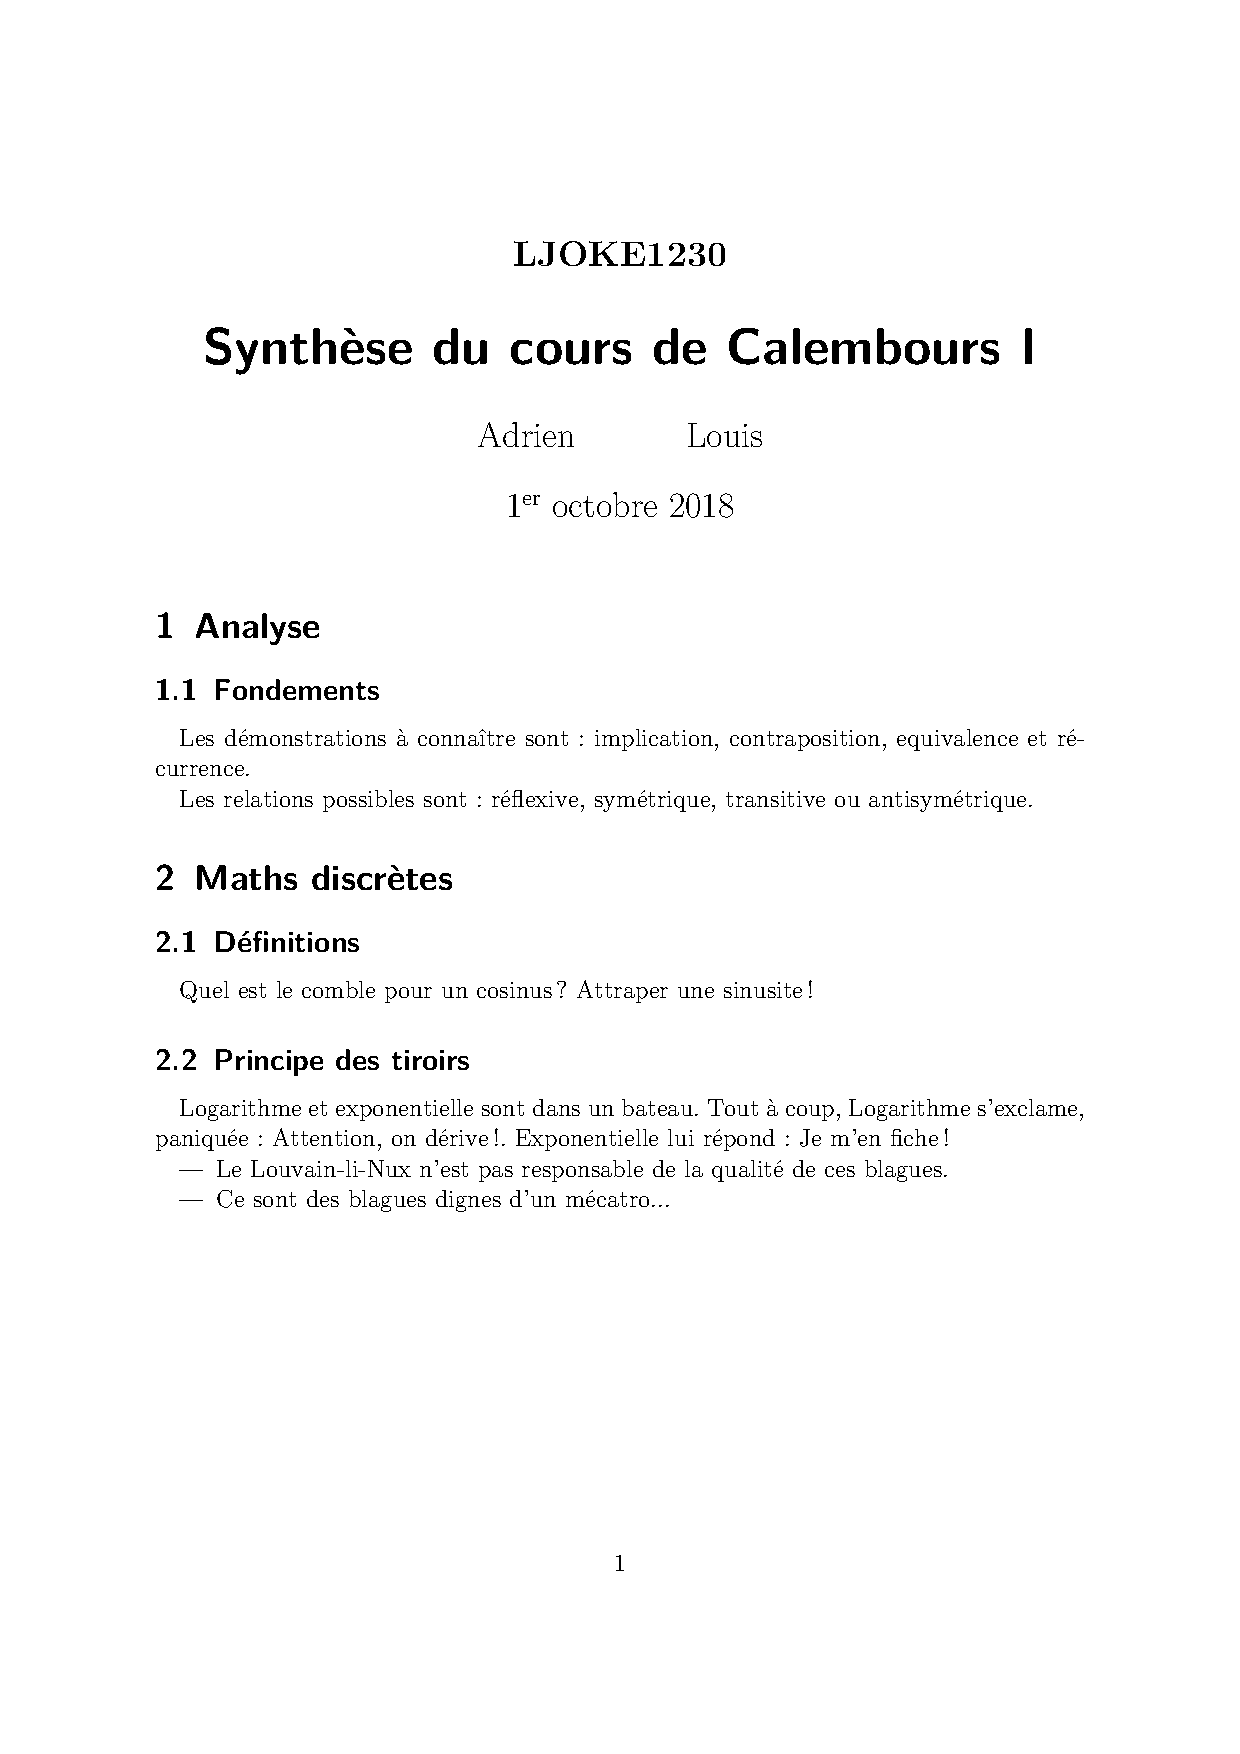
\includegraphics[height=7cm,trim={1.5cm 8cm 1.5cm 3cm},clip]{exercices/1/build_latex/main.pdf}}
\end{center}

\end{frame}

\begin{frame}[fragile]{Premier exercice (solution)}
\begin{center}
Lien Overleaf de la solution du premier exercice \url{https://www.overleaf.com/read/cgsxdzhjrknb}
\end{center}

\end{frame}

%-----------------------
\subsection{Notes de bas de page}
\begin{frame}[fragile]
  \frametitle{Notes de bas de page}
  La commande \lstinline|\footnote{}| permet d'ajouter une note de bas de page:
  \begin{lstlisting}[style=nonumbers]
It's the ship that made the Kessel\footnote{Kessel is a planet in the Outer Rim} run in less than twelve parsecs\footnote{Whatever that means...}.

She's fast enough for you, old man.
  \end{lstlisting}
  \begin{minipage}{\textwidth}
    It's the ship that made the Kessel\footnote{Kessel is a planet in the Outer Rim} run in less than twelve parsecs\footnote{Whatever that means...}.

    She's fast enough for you, old man.
  \end{minipage}
\end{frame}

%-----------------------
\subsection{Les polices}

\begin{frame}[fragile]{Changer la fonte de la police}

\begin{itemize}
    \item Mise en emphase:
    \begin{center}
    \begin{tabular}{ll}
    \lstinline|\emph{Emphase}| & Mise en \emph{emphase} du texte
    \end{tabular}
    \end{center}
\item Style de police
\begin{center}
\begin{tabular}{ll}
\lstinline|\textbf{Gras}| & \textbf{Gras} \\
\lstinline|\textit{Italique}| & \textsl{Italique} \\
\lstinline|\textsc{Petites majuscules}| & \textsc{Petites majuscules} \\
\lstinline|\texttt{Machine à écrire}| & \texttt{Machine à écrire} \\
\lstinline|\textrm{Serif (par défaut)}| & \textrm{Serif (par défaut)}
\end{tabular}
\end{center}
\end{itemize}
\end{frame}

\subsection{Divers}
\begin{frame}[fragile]{Divers}
  \frametitle{Divers}
  \begin{itemize}
  \item Caractères spéciaux utilisés par \LaTeX

  \begin{tabular}{cccccccccc}
  \lstinline|\$| & \lstinline|\&| & \lstinline|\%| & \lstinline|\#| & \lstinline|\_| & \lstinline|\{| & \lstinline|\}| & \lstinline|\~{}| & \lstinline|\^{}| & \lstinline|\textbackslash| \\
  \$ & \& & \% & \# & \_ & \{ & \} & \~{} & \^{} & \textbackslash
  \end{tabular}

 \item Tirets
   \begin{tabular}{llp{0.5\textwidth}}
     \lstinline|-| & court & Jean-Patrick\\
     \lstinline|--| & moyen ou semi-cadratin & 1984--2015\\
     \lstinline|---| & cadratin & le \LaTeX{} --- c'est chouette --- a été créé par Leslie Lamport\\
   \end{tabular}

    \item Autres caractères (attention, certains nécessitent la présence du package \texttt{babel (french)})
    \begin{itemize}
        \item \lstinline|M\up{me}| pour M\up{me}
        \item \lstinline|1\ier{} 2\ieme{}| pour 1\ier{} et 2\ieme{}
        \item \lstinline|\no \No| pour \no et \No
    \end{itemize}
 \end{itemize}
\end{frame}



%-----------------------
\section{Les environnements flottants}
\subsection{Les figures}

\begin{frame}[fragile]
  \frametitle{Figures I}
  \begin{itemize}

  \item Utilisation du package \lstinline|\usepackage{graphicx}|
  \item Insertion de l'image avec \lstinline|\includegraphics[options]{filename.ext}|

  \item \textbf{Non-flottant}

    Référencement par ``ci-dessous'', \dots
    \begin{lstlisting}[style=nonumbers]
\begin{center}
  \includegraphics{image.jpg}
\end{center}
    \end{lstlisting}

  \item \textbf{Flottant}
      \begin{itemize}
          \item Environnement \lstinline|figure|
          \item Ajout d'une référence par \lstinline|\label{...}|
        \item Référencement par \lstinline|voir figure \ref{fig:graphique}|
        \item Ajout d'une légende par \lstinline|\caption{...}|
    \end{itemize}
    \begin{lstlisting}[style=nonumbers]
\begin{figure}
  \centering
  \includegraphics{graph.png}
  \caption{Voici un beau graphique}
  \label{fig:graphique}
\end{figure}
    \end{lstlisting}
\end{itemize}
\end{frame}

\begin{frame}[fragile]
  \frametitle{Référencer des éléments du texte}
  Pour faire référence à une page, section, figure, table, équation mathématique, \dots:
  \begin{itemize}
    \item Mettre une étiquette (label) à l'endroit à référencer
      \begin{itemize}
        \item \lstinline|\label{identifiant}|.
      \end{itemize}
    \item Mettre une référence à cette étiquette :
      \begin{itemize}
        \item \lstinline|\ref{identifiant}| pour le numéro de section, figure, table, équation;
        \item \lstinline|\pageref{identifiant}| pour le numéro de page;
      \end{itemize}
  \end{itemize}
  \begin{columns}
    \begin{column}{0.5\textwidth}
      \begin{lstlisting}[style=nonumbers]
  \label{ref}
  Nous sommes section \ref{ref},
  page \pageref{ref},
      \end{lstlisting}
    \end{column}
    \begin{column}{0.5\textwidth}
      \label{ref:id}
      \par{}Nous sommes section~\ref{ref:id},
      page~\pageref{ref:id},
    \end{column}
  \end{columns}
\end{frame}

\begin{frame}[fragile]\
    \frametitle{Figures II}
    \begin{itemize}

  \item \textbf{Scaling}
    \begin{lstlisting}[style=nonumbers]
\includegraphics[width=0.7\textwidth]{image.jpg} % Largeur dépendant du texte
\includegraphics[height=4cm]{image.jpg} % Hauteur de 4cm
\includegraphics[scale=0.5]{image.png} % taille de l'image / 2
    \end{lstlisting}

  \vspace{2em}
\end{itemize}

\end{frame}


\begin{frame}[fragile]{Exemple de figure}

\begin{columns}
\begin{column}{0.5\textwidth}
\begin{lstlisting}[style=nonumbers]

Sur la figure \ref{fig:uclLogo}, vous pouvez
voir le logo UCLouvain mis a 50\%
de la largeur du texte.

\begin{figure}
    \centering
    
\includegraphics[width=0.50\textwidth]{logo-uclouvain.eps}
    \caption{Voici le logo UCLouvain}
    \label{fig:uclLogo}
\end{figure}
\end{lstlisting}
\end{column}
\begin{column}{0.5\textwidth}
Sur la figure \ref{fig:uclLogo}, vous pouvez voir le logo UCLouvain
mis a \SI{50}{\percent} de la largeur du texte.

\begin{figure}[!ht]
    \centering
    
\includegraphics[width=0.50\textwidth]{logo-uclouvain.pdf}
    \caption{Voici le logo UCLouvain}
    \label{fig:uclLogo}
\end{figure}
\end{column}
\end{columns}

\end{frame}


\subsection{Les tableaux}
\begin{frame}[fragile,allowframebreaks]
  \frametitle{Tableaux}
  \begin{itemize}
    \item \textbf{Code}
      \begin{lstlisting}[style=nonumbers]
\begin{tabular}{<colonnes>}
  <lignes>
\end{tabular}
      \end{lstlisting}
      \begin{itemize}
          \item Définition de l'alignement des <colonnes> par :
              \begin{itemize}
                  \item un \lstinline|l| pour aligner à gauche (\textit{left})
                  \item un \lstinline|c| pour centrer (\textit{center})
                  \item un \lstinline|r| pour aligner à droite (\textit{right})
                  \item un \lstinline|p{<largeur>}| pour un texte justifié sur une largeur donnée
              \end{itemize}
          \item Une ligne verticale est tracée par \lstinline|||
          \item Le contenu des <lignes> est séparé par colonne grâce à des \lstinline|&|
          \item Une <ligne> se termine par \lstinline|\\|
          \item Une ligne horizontale est tracée par \lstinline|\hline|
      \end{itemize}\framebreak
    \item \textbf{Exemple}
    \begin{lstlisting}
\begin{tabular}{|lcrp{0.25\textwidth}|}
  \hline
  Gauche & Centré & Droite & Justifié\\
  \hline
  a & b & c & Le texte est trop long.\\
  1 & 2 & 3 & Il passe donc à la ligne suivante.\\
  \hline
\end{tabular}
        \end{lstlisting}
      \item \textbf{Rendu}
    \begin{table}[!ht]
    \centering
    \begin{tabular}{|lcrp{0.25\textwidth}|}
      \hline
      Gauche & Centré & Droite & Justifié\\
      \hline
      a & b & c & Le texte est trop long.\\
      1 & 2 & 3 & Il passe donc à la ligne suivante.\\
      \hline
    \end{tabular}
    \end{table}
    \framebreak

      \item \textbf{Non-flottant}

    Référencement par ''ci-dessous'', \dots
    \begin{lstlisting}[style=nonumbers]
\begin{center}
    \begin{tabular}{...}
        ...
    \end{tabular}
\end{center}
    \end{lstlisting}

  \item \textbf{Flottant}
      \begin{itemize}
          \item Environnement \lstinline|table|
        \item Référencement par \lstinline|voir tableau \ref{tab:data}|
    \end{itemize}
    \begin{lstlisting}
\begin{table}
  \centering
  \begin{tabular}{...}
    ...
  \end{tabular}
  \caption{Voici un beau tableau}
  \label{tab:data}
\end{table}
    \end{lstlisting}


  \end{itemize}
\end{frame}



\begin{frame}[fragile]{Exemple de tableau}
\begin{footnotesize}
\begin{lstlisting}[style=nonumbers]
\begin{table}
  \begin{center}
    \begin {tabular}{|l||c|} %% 2 columns
      \hline
      \textit{Inventaire} & \textbf{Nombre} \\
      \hline
      Chemises  & 4   \\
      Pulls     & 12  \\
      Pantalons & 1   \\
      \hline
    \end{tabular}
    \caption{Tableau relatif a l'inventaire}
  \end{center}
\end{table}
\end{lstlisting}
\end{footnotesize}
\begin{center}
\fbox{\includegraphics[width=0.6\textwidth]{table.jpg}}
\end{center}
\end{frame}

\subsection{Exercice 2}
\begin{frame}[fragile]{Deuxième exercice}
\begin{center}
\fbox{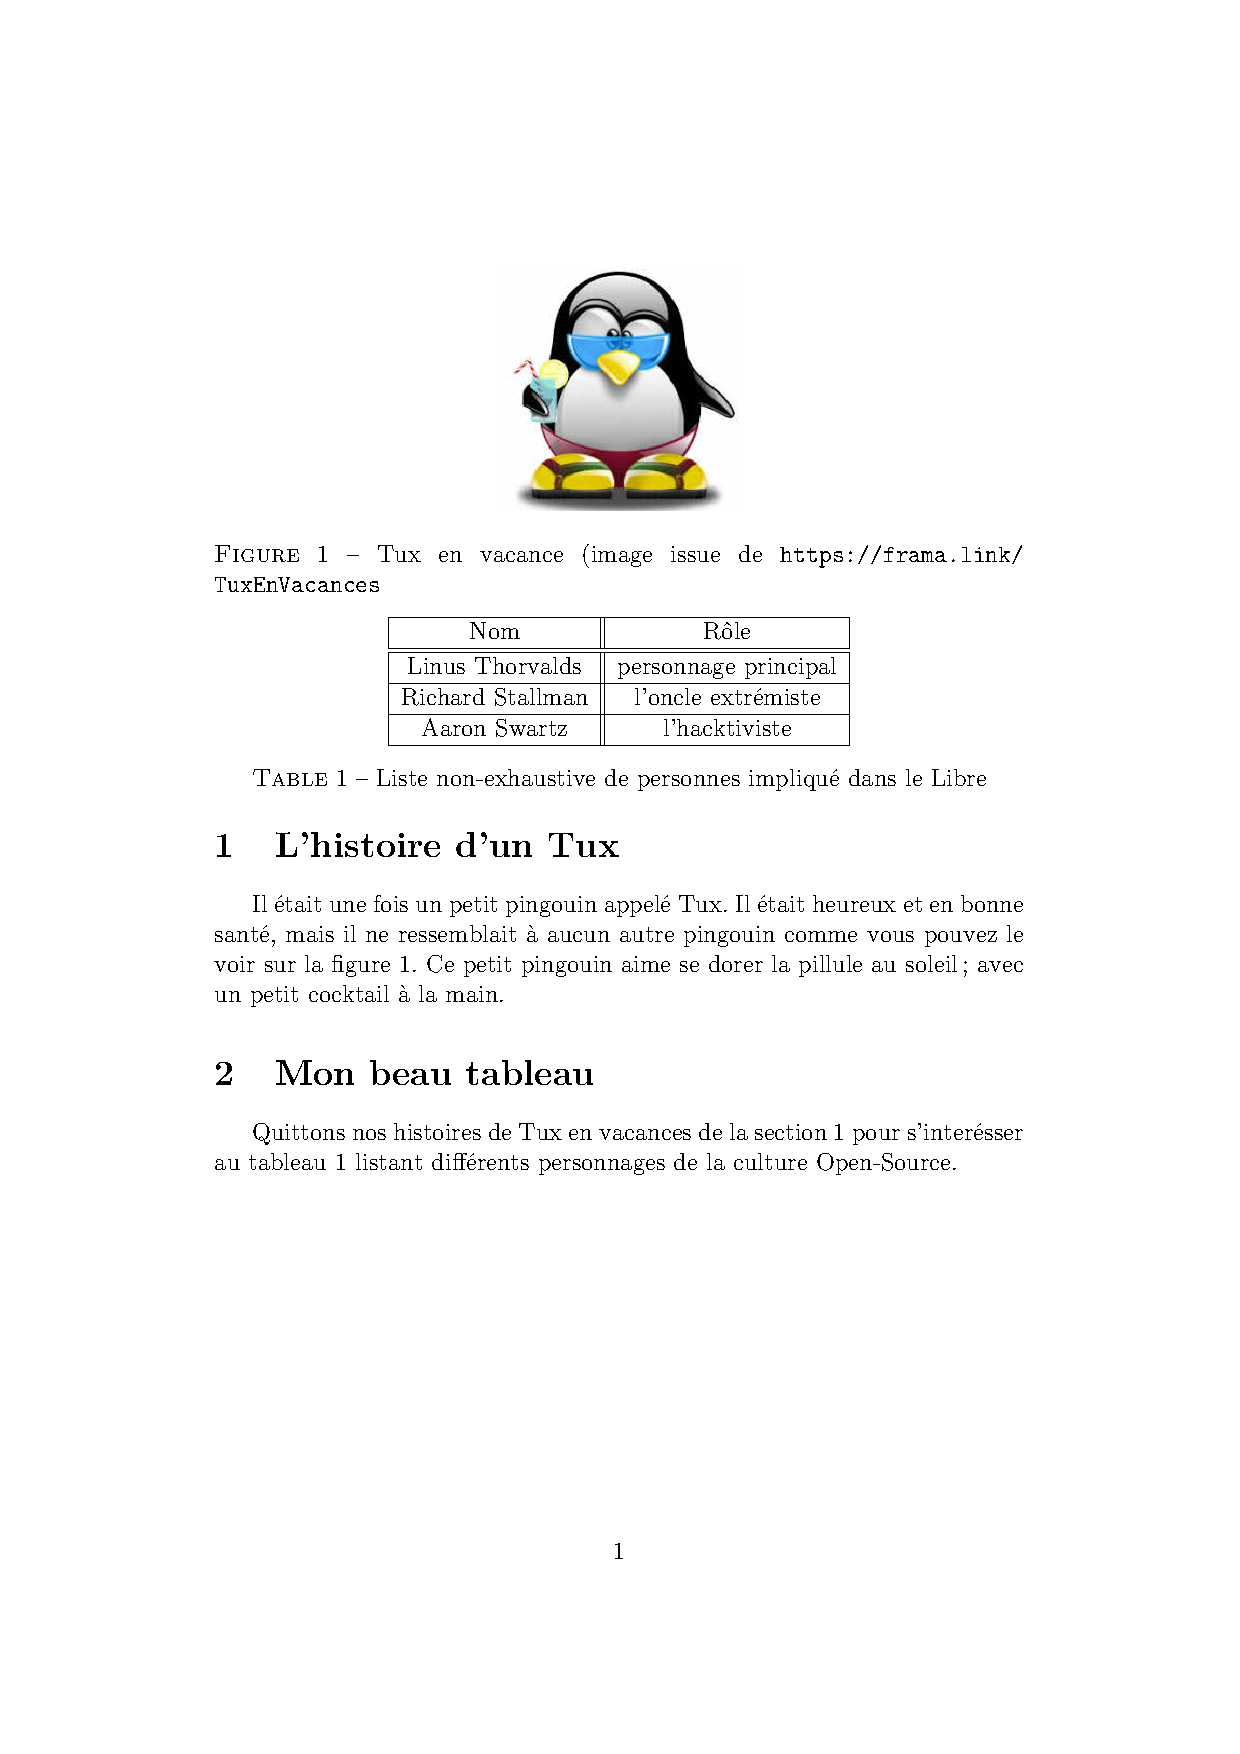
\includegraphics[height=7cm,trim={2cm 8cm 2cm 4cm},clip]{exercices/2/build_latex/main.pdf}}
\end{center}
\end{frame}

\begin{frame}[fragile]{Deuxième exercice (solution)}
\begin{center}
Lien Overleaf de la solution du deuxième exercice \url{https://www.overleaf.com/read/dmcqrmdjwmdw}
\end{center}

\end{frame}



%%%%%%%%%%%%%%%%%%%%%%%%%%%
\section{Bibliographie}

%-------------------
\subsection{Bibliographie}
\begin{frame}[fragile]
  \frametitle{\insertsubsection}
  \begin{itemize}
    \item Avec \LaTeX{}, la bibliographie est séparée du reste dans un fichier \texttt{.bib} (par exemple: \texttt{biblio.bib}).
    \item L'utilisation d'une bibliographie requièrent les paquets suivants :
    \begin{itemize}
    \item \lstinline|\usepackage[backend=bibtex]{biblatex}|
    \item \lstinline|\usepackage{csquotes}|.
    \end{itemize}
    \item On utilise le fichier \texttt{biblio.bib} dans le document via la commande \lstinline|\bibliography{biblio.bib}| (dans l'en-tête du document).
    \item On cite un document avec la commande \lstinline|\cite{identifiant}|. Cet identifiant est repris dans le fichier \texttt{.bib}.
    \item On affiche la bibliographie à l'endroit souhaité avec la commande \lstinline|\printbibliography|.
\end{itemize}
\end{frame}

\begin{frame}[fragile,allowframebreaks]
\frametitle{Structure du fichier \texttt{.bib}}
\begin{itemize}
    \item Pour chaque référence bibliographique, on ajoute une entrée au fichier. Exemple avec un article de Laurent Francis:
      \begin{lstlisting}[style=nonumbers]
@inproceedings{ray2017challenges,
    title={Challenges of monolithic integration for SiGe MEMS technology},
    author={Ray Chaudhuri, Ashesh and Severi, S and Helin, P and Francis, Laurent and Tilmans, HAC},
    booktitle={15th IEEE Sensors Conference, SENSORS 2016},
    year={2017}
}
      \end{lstlisting}
    Et un autre qui fit beaucoup de bruit:
    \begin{lstlisting}[style=nonumbers]
@article{lemaitre1934evolution,
    title={Evolution of the expanding universe},
    author={Lema{\^\i}tre, Georges},
    journal={Proceedings of the National Academy of Sciences},
    volume={20}, number={1}, pages={12--17},
    year={1934},
    publisher={National Acad Sciences}
}
    \end{lstlisting}
    \framebreak
    Et encore un autre, que nous ne citerons pas:
    \begin{lstlisting}[style=nonumbers]
@article{de1966functions,
  title={Functions of lysosomes},
  author={De Duve, Christian and Wattiaux, Robert},
  journal={Annual review of physiology},
  year={1966},
  publisher={Annual Reviews 4139 El Camino Way, PO Box 10139, Palo Alto CA 94303-0139}
}
    \end{lstlisting}
  \end{itemize}
\end{frame}

\begin{frame}[fragile]
    \frametitle{Exporter des \texttt{.bib}}
    \framesubtitle{Par exemple sur Google Scholar :}
    \begin{center}
    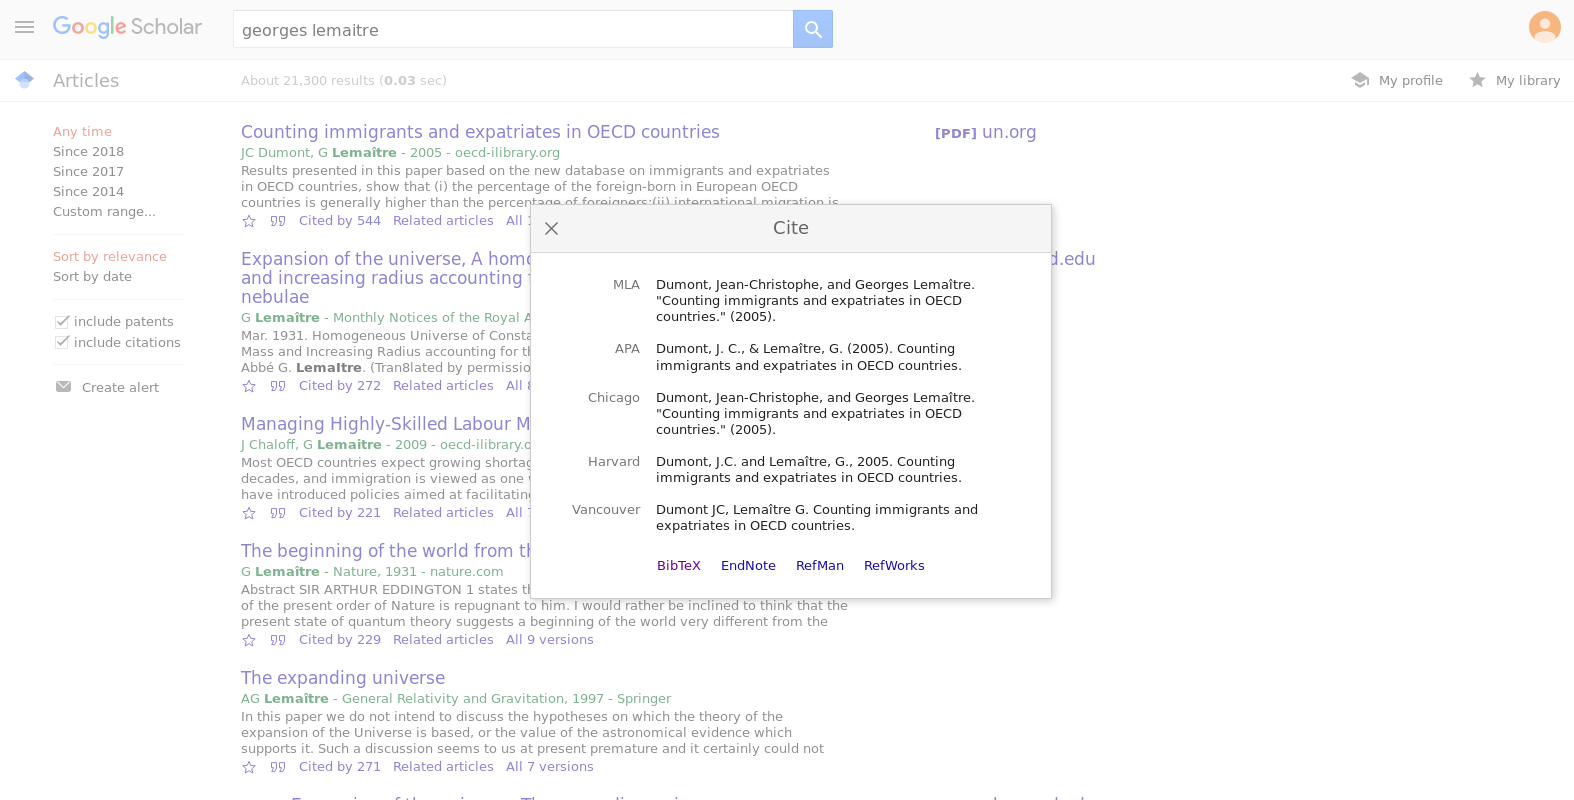
\includegraphics[width=\textwidth]{img/scholar.png}
    \end{center}
\end{frame}

\begin{frame}[fragile]
    \frametitle{Style de bibliographie}
    \begin{itemize}
        \item Le style est défini lors de l'appel du paquet \lstinline|\usepackage[style=ieee]{biblatex}|
        \item Les différents styles sont:
        \begin{itemize}
            \item \texttt{apa}, American Psychological Association;
            \item \texttt{chicago-authordate}, Chicago Style;
            \item \texttt{ieee}, Institute of Electrical and Electronics Engineers (IEEE).
        \end{itemize}
        \item Pour plus de style de bibliographie, voir \url{https://www.overleaf.com/learn/latex/Biblatex_citation_styles} et Google.
    \end{itemize}
\end{frame}

\begin{frame}[fragile]
    \frametitle{Exemple}
    \begin{lstlisting}[style=nonumbers,mathescape]
\documentclass[11pt]{scrartcl}
\usepackage[utf8]{inputenc}
\usepackage[T1]{fontenc}
\usepackage[style=authoryear]{biblatex}
\usepackage{csquotes}
\usepackage[french]{babel}
\$\color{blue}{\texttt{bibliography}}$
\begin{document}
Lorem ipsum dolor sit amet\$\color{blue}{\texttt{cite}}${ray2017challenges}, consectetuer adipiscing elit.
Ut purus elit, vestibulum ut, placerat ac, adipiscing vitae, felis. Curabitur
dictum gravida mauris. Nam arcu libero, nonummy eget, consectetuer id, vulputate
a, magna. Donec vehicula augue eu neque. Pellentesque habitant morbi tristique
senectus et netus et malesuada fames ac turpis egestas. Mauris ut leo. Cras
viverra\$\color{blue}{\texttt{cite}}${lemaitre1934evolution} metus rhoncus sem. Nulla et lectus vestibulum
urna fringilla ultrices.
\$\color{blue}{\texttt{nocite}}${de1966functions}
\$\color{blue}{\texttt{printbibliography}}$
\end{document}
    \end{lstlisting}
    \begin{itemize}
        \item La commande \lstinline|\nocite{}| permet d'inclure dans la bibliographie un élément dans la bibliographie qui n'a pas été cité dans le texte.
    \end{itemize}
\end{frame}

\begin{frame}[fragile]
    \frametitle{Compilation}
    \begin{itemize}
        \item Pour \textbf{TeXMaker}
        \begin{itemize}
            \item Options $\rightarrow$ Configurer Texmaker $\rightarrow$ Compil rapide $\rightarrow$ Sélectionner ``PdfLaTex + BibLaTeX + PdfLaTeX (2x) + Voir pdf''
        \end{itemize}
        \item Pour \textbf{Overleaf}
        \begin{itemize}
            \item Fonctionne déjà dans la compilation de base.
        \end{itemize}
    \end{itemize}
\end{frame}

\begin{frame}[fragile]
    \frametitle{Troisième exercice}
    \begin{center}
        Compiler l'exemple de bibliographie et ajouter une référence depuis Google Scholar.\vspace{0.5cm}
        \fbox{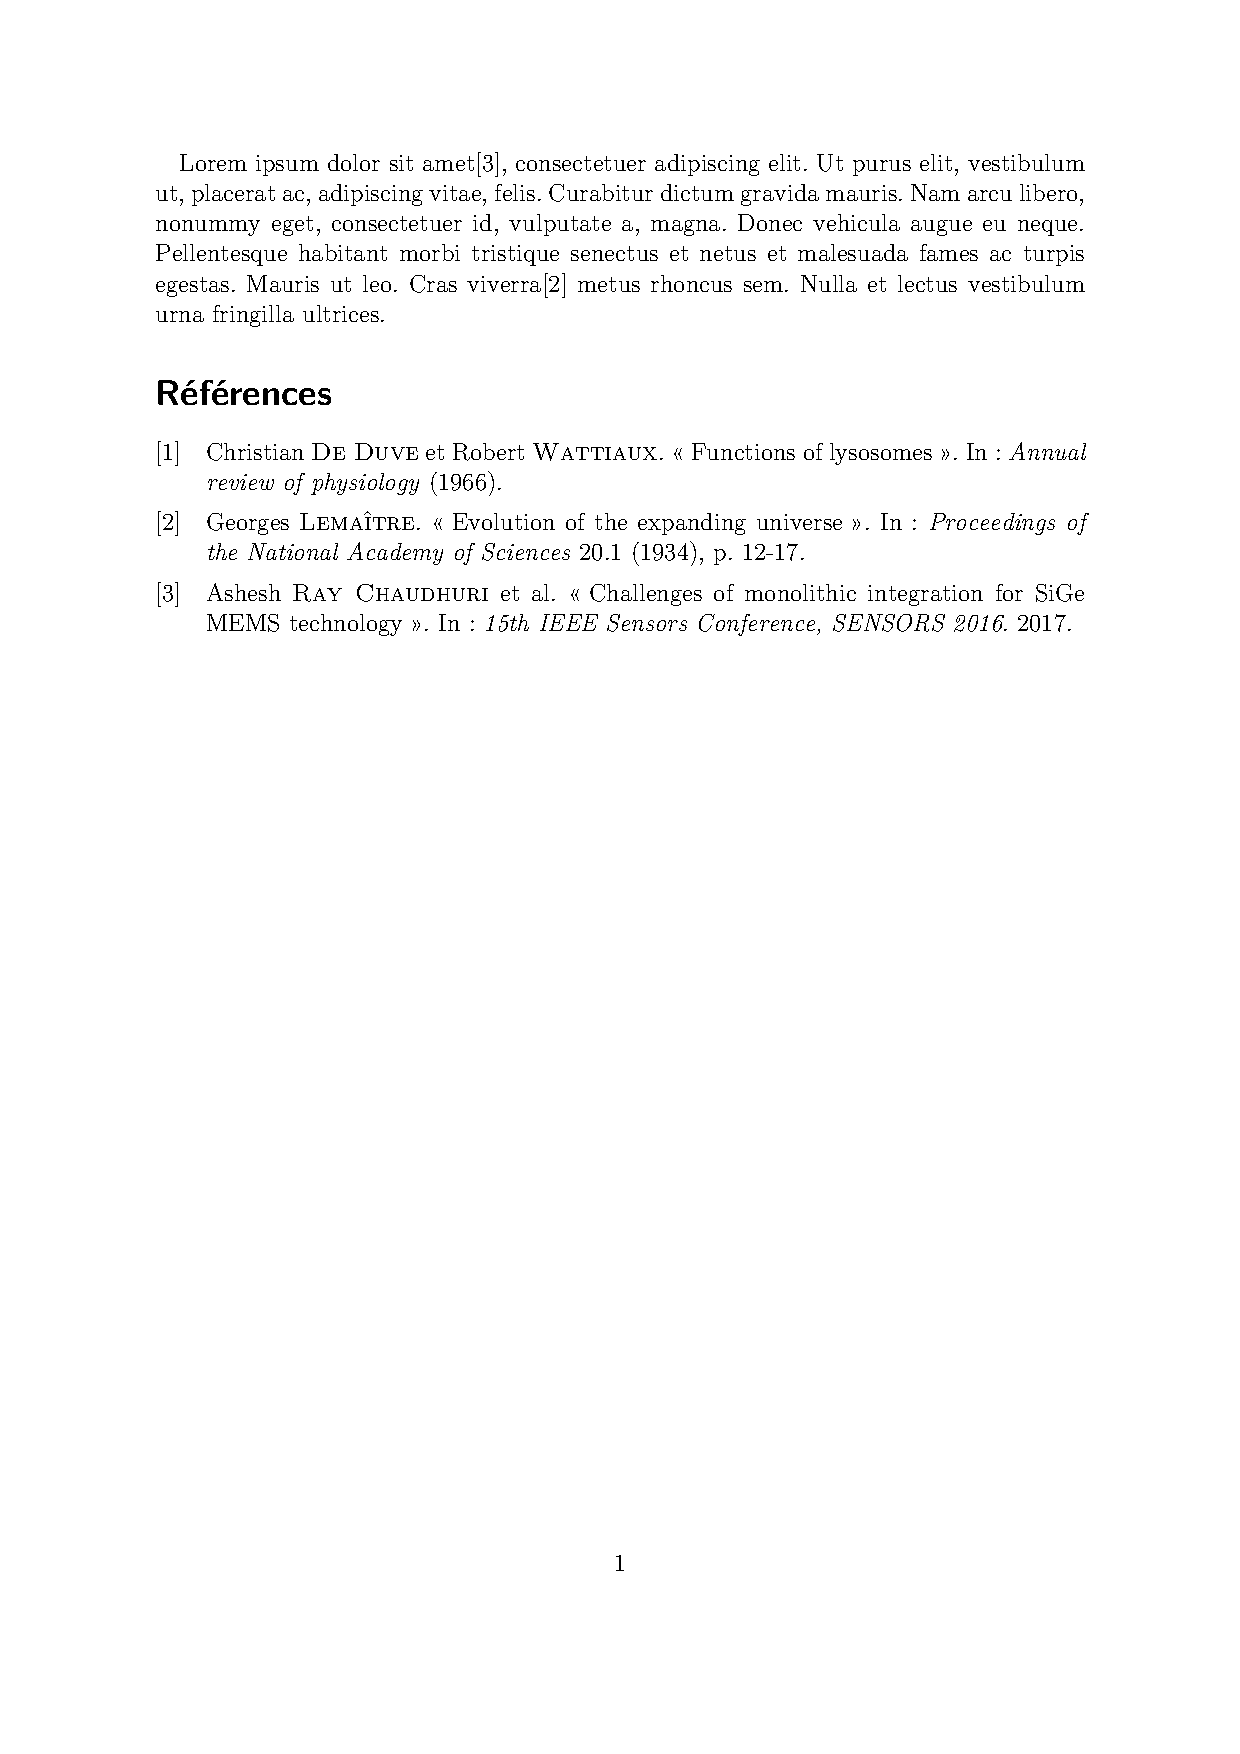
\includegraphics[width=0.8\textwidth,trim={2cm 18cm 2cm 2cm},clip]{exercices/bib/build_latex/main.pdf}}
    \end{center}
\end{frame}
\begin{frame}[fragile]{Troisième exercice (solution)}
\begin{center}
Lien Overleaf de la solution du troisième exercice \url{https://www.overleaf.com/read/pstswcfgbsyg}
\end{center}
\end{frame}


%-------------------
\subsection{Découpe d'un projet en fichiers}
\begin{frame}[fragile]
  \frametitle{Découpe d'un projet en fichiers}
  \begin{itemize}
    \item Si vous travaillez sur un projet de moyenne ou grande envergure, il vaut la peine de le découper en plusieurs fichiers
    \item Cela accélère la recompilation et permet une séparation plus claire entre les sections
    \item Par exemple, un article pourrait avoir un fichier par section:
    \begin{itemize}
      \item \texttt{main.tex} contient la structure et l'en-tête du projet;
      \item \texttt{intro.tex} contient l'introduction et les remerciements;
      \item \texttt{section1.tex} contient la première section et son titre;
      \item \texttt{section2.tex} contient la deuxième section et son titre;
      \item \dots
    \end{itemize}
    \item L'inclusion dans fichier dans un autre se fait via la commande \lstinline|\input{}|.
  \end{itemize}
\end{frame}

\begin{comment}
\begin{frame}[fragile]
  \frametitle{Découpe d'un projet en fichiers}
  \framesubtitle{input et include}
  \begin{itemize}
    \item Deux commandes permettent l'inclusion d'un fichier dans un autre: \lstinline|\input{}| et \lstinline|\include{}|
    \item On leur donne en argument le nom du fichier sans le \texttt{.tex}
    \item \lstinline|\input{}| \og{}copie\fg{} le document littéralement
    \item \lstinline|\include{}| termine la page courante, copie le document, puis termine la page courante à nouveau
    \item \lstinline|\input{}| peut se trouver n'importe où, y compris dans le préambule, tandis que \lstinline|\include{}| doit se trouver dans le corps du document
    \item \lstinline|\include{}| accélère la compilation du document, car cela permet de ne recompiler que ce qui a été modifié
    \item La commande \lstinline|\includeonly{doc1,doc2,...}| permet de restreindre les documents à inclure
  \end{itemize}
\end{frame}
\end{comment}

\begin{frame}[fragile]
    \frametitle{Découpe d'un projet en fichiers}
    \framesubtitle{Exemple de l'article}
    \begin{columns}
        \begin{column}{0.5\textwidth}
            Dans \texttt{main.tex}
            \begin{lstlisting}[style=nonumbers, mathescape]
\documentclass[a4paper]{scrartcl}
\usepackage[utf8]{inputenc}
\usepackage[T1]{fontenc}
\usepackage[french]{babel}

\begin{document}
\maketitle
\tableofcontents

\input{intro.tex}
  \input{$\color{black}{\texttt{section}}$1.tex}
  \input{$\color{black}{\texttt{section}}$2.tex}
  ...
\end{document}
            \end{lstlisting}
        \end{column}
        \begin{column}{0.5\textwidth}
            Dans \texttt{intro.tex}
            \begin{lstlisting}[style=nonumbers]
\begin{center}
  Je dédie cet article à mon chat.
  Tu nous a quitté trop vite, Dragibus.
  Repose en paix.
\end{center}
            \end{lstlisting}
      
            Dans \texttt{section1.tex}
            \begin{lstlisting}[style=nonumbers]
\section{Le Louvain-li-Nux}
  Le Louvain-li-Nux est un kot à projet
  de Louvain-la-Neuve.
  ...
            \end{lstlisting}
      
            Dans \texttt{section2.tex}
            \begin{lstlisting}[style=nonumbers]
\section{Le Kotangente}
  Le Kotangente est kot ami du
  Louvain-li-Nux.
  ...
            \end{lstlisting}
        \end{column}
    \end{columns}
\end{frame}

%%%%%%%%%%%%%

%-----------------------

\section{Mathématiques}

\subsection{Écrire des mathématiques}
\begin{frame}[fragile]{L'environnement mathématique}
\framesubtitle{Inclure des formules dans le texte}
\begin{itemize}
    \item On peut ouvrir un environnement mathématique entre deux symboles \textbf{\$}.

\begin{center}
  \begin{tabular}{lll}
    \lstinline|$x + 1 = 2$| & $x + 1 = 2$\\
    \medskip
    \lstinline|$\frac{1}{x}$| & $\frac{1}{x}$\\
  \end{tabular}
\end{center}
    \item Les opérateurs et symboles, comme les autres commandes, commencent par \textbf{\textbackslash}, sauf \lstinline|+, -, /, ^,| et \lstinline|_|
    \begin{center}
        \begin{tabular}{llr}
            \lstinline|$a^{11}$| & $a^{11}$ & Good \\
            \lstinline|$a^11$| & $a^11$ & Bad ! \\
            \lstinline|$\sin(x)$| & $\sin(x)$ & Good \\
            \lstinline|$sin(x)$| & $sin(x)$ & Bad !\\
            \lstinline|$\frac{\Theta}{\sqrt{\beta}}$| & $\frac{\Theta}{\sqrt{\beta}}$ & Very good !
        \end{tabular}
    \end{center}
    \item Les packages \lstinline|amsmath| et \lstinline|amssymb| apportent beaucoup d'environements et symboles supplémentaires très utiles, à inclure par défaut.
\end{itemize}
\end{frame}

\begin{frame}[fragile]{L'environnement mathématique}
\framesubtitle{Inclure des formules centrées hors du texte}

\begin{itemize}
\item On peut aussi ajouter une formule mathématique centrée hors du texte entre \lstinline|\[ ... \]|.
\vspace{0.5cm}
\begin{columns}
  \begin{column}{0.45\textwidth}
    \begin{lstlisting}[style = nonumbers]
L'expression $\sin(x)$ peut s'écrire de différents manières. En effet, il a été démontré que

\[
  \sin(x) =
  \frac{e^{iz} - e^{-iz}}{2i}
\]

avec $i$ étant l'unité imaginaire.
    \end{lstlisting}
  \end{column}
  \begin{column}{0.45\textwidth}
    L'expression $\sin(x)$ peut s'écrire de différents manières. En effet, il a été démontré que

    \[ \sin(x) = \frac{e^{iz} - e^{-iz}}{2i} \]

    avec $i$ étant l'unité imaginaire.
  \end{column}

\end{columns}

\end{itemize}
\end{frame}
\subsection{Matrices}
\begin{frame}[fragile]{Matrices}
  \begin{itemize}
    \item Les matrices s'écrivent avec l'environnement \lstinline|matrix| (fonctionnement semblable à \lstinline|tabular|).
      \begin{columns}
        \begin{column}{0.45\textwidth}
          \begin{lstlisting}[style=nonumbers]
\[
  \begin{matrix}
    \alpha & \beta \\
    \gamma & \delta \\
  \end{matrix}
\]
          \end{lstlisting}
        \end{column}
        \begin{column}{0.45\textwidth}
          \[\begin{matrix}
            \alpha & \beta \\
            \gamma & \delta \\
            \end{matrix}\]
        \end{column}
      \end{columns}
    \item On ajoute des délimiteurs avec \lstinline|pmatrix|,\lstinline|vmatrix|,\ldots{}
      \begin{columns}
        \begin{column}{0.45\textwidth}
          \begin{lstlisting}[style=nonumbers]
\[
  \begin{pmatrix}
    a + b & c \\
    d & e + f \\
  \end{pmatrix}
\]
          \end{lstlisting}
        \end{column}
        \begin{column}{0.45\textwidth}
          \[\begin{pmatrix}
            a + b & c \\
            d & e + f \\
            \end{pmatrix}\]
        \end{column}
      \end{columns}
    \item Les différents délimiteurs sont
      \begin{center}
        \begin{tabular}{llllll}
            \lstinline|bmatrix| & [ ] & \lstinline|Bmatrix| & \{ \} & \lstinline|pmatrix| & ( ) \\
            \lstinline|vmatrix| & | | &	\lstinline|Vmatrix| & || ||
        \end{tabular}
      \end{center}
    \end{itemize}
\end{frame}

\begin{frame}[fragile]
    \frametitle{Les délimiteurs}
    \begin{itemize}
        \item Par défaut \LaTeX utilise des parenthèses de taille standard, ne s'adaptant pas au contenu qu'elles contiennent.
        \begin{lstlisting}[style=nonumbers]
\[ ( \frac{x^2}{y^3} ) \]
\end{lstlisting}
\[ (\frac{x^2}{y^3}) \]
        \item La solution ? Les commandes \lstinline|\left...| et \lstinline|\right...| permettent d'adapter automatiquement la taille des parenthèses.
        \begin{lstlisting}[style=nonumbers]
\[ \left( \frac{x^2}{y^3} \right) \]
\end{lstlisting}
\[ \left( \frac{x^2}{y^3} \right) \]
        \item Fonctionne aussi avec \lstinline|\left\{ \right\}| ou \lstinline|\left[ \right]|
\[ \left\{\frac{x^2}{y^3}\right\} \qquad \left[\frac{x^2}{y^3}\right] \]
    \end{itemize}
\end{frame}





\subsection{Formules numérotées}
\begin{frame}[fragile,allowframebreaks]{Formules numérotées}

\begin{itemize}
    \item L'environnement \lstinline|equation| permet d'écrire des équations numérotées.
    \begin{columns}
        \begin{column}{0.5\textwidth}
            \begin{lstlisting}[style=nonumbers]
\begin{equation}
    c^2 = a^2 + b^2
\end{equation}
\end{lstlisting}
        \end{column}
        \begin{column}{0.5\textwidth}
            \begin{equation}
                c^2 = a^2 + b^2
            \end{equation}
        \end{column}
    \end{columns}

    \item L'environnement \lstinline|align| permet d'écrire des équations alignées et numérotées. \lstinline|align*| aligne plusieurs équations sans les numéroter.
    \item On peut ne pas numéroter une équation en plaçant \lstinline|\nonumber| à la fin de la ligne.
\begin{columns}
    \begin{column}{0.5\textwidth}
    \begin{lstlisting}[style = nonumbers]
I like trains and the equations
\begin{align}
  e^{i\pi} + 1 & = 0\\
  f(t) & = A\cos(\omega t + \phi) \nonumber
\end{align}
I also know that
\begin{align*}
  1 + 1 & = 2\\
  2 + 3 & = 5
\end{align*}
\end{lstlisting}
  \end{column}
  \begin{column}{0.5\textwidth}
I like trains and the equations
\begin{align}
  e^{i\pi} + 1 & = 0\\
  f(t) & = A\cos(\omega t + \phi) \nonumber
\end{align}
I also know that
\begin{align*}
  1 + 1 & = 2\\
  2 + 3 & = 5
\end{align*}
  \end{column}

\end{columns}
\framebreak
    \item Utilisation de l'environnement \lstinline|aligned| pour faire un système d'équation (utilisation semblable à \lstinline|align|).
    \begin{columns}
            \begin{column}{0.5\textwidth}
            \begin{lstlisting}[style=nonumbers]
\[
    \left\{
        \begin{aligned}
         x^2 + y &= 3 \\
         \frac{y}{x} &= 0.42
        \end{aligned}
    \right.
\]
            \end{lstlisting}
        \end{column}
        \begin{column}{0.5\textwidth}
            \[ \left\{\begin{aligned}
                x^2 + y &= 3 \\
                \frac{y}{x} &= 0.42
            \end{aligned}\right. \]
        \end{column}

    \end{columns}
\end{itemize}
\end{frame}

\subsection{Les maths et les polices}
\begin{frame}[fragile]{Les maths et les polices}
\begin{itemize}
    \item Parfois, certaines variables sont composées de plusieurs lettres. On doit utiliser des polices différentes comme \lstinline|\mathrm| ou \lstinline|\mathsf|. \lstinline|\mathcal| produit des lettres \og calligraphiques \fg{}.
    \begin{center}
            \begin{tabular}{lll}
                \lstinline|$Var(x)$| & $Var(x)$ & Bad ! \\
                \lstinline|$\mathrm{Var}(x)$| & $\mathrm{Var}(x)$ & Good \\
                \lstinline|$F_{machine}$| & $F_{machine}$ & Bad ! \\
                \lstinline|$F_\mathrm{machine}$| & $F_\mathrm{machine}$ & Good \\
                \lstinline|$\mathcal{M}$| & $\mathcal{M}$ &
            \end{tabular}
    \end{center}

    \item Les ensembles s'écrivent à l'aide de la police \lstinline|\mathbb|.
    \begin{center}
        \begin{tabular}{cccc}
        \lstinline|$\mathbb{N}$| & $\mathbb{N}$ & \lstinline|$\mathbb{Z}$| & $\mathbb{Z}$ \\
        \lstinline|$\mathbb{D}$| & $\mathbb{D}$ & \lstinline|$\mathbb{Q}$| & $\mathbb{Q}$ \\
        \lstinline|$\mathbb{N}$| & $\mathbb{R}$ & \lstinline|$\mathbb{C}$| & $\mathbb{C}$
        \end{tabular}
    \end{center}
\end{itemize}
\end{frame}

\subsection{Large Operators}
\begin{frame}[fragile]{Large Operators}
\begin{itemize}
    \item Voici quelques opérateurs utiles:
    \begin{center}
        \begin{tabular}{lll}
        \lstinline|\min_{x \in \mathbb{R}}| & $\min_{x \in \mathbb{R}}$ & $\displaystyle\min_{x \in \mathbb{R}}$ \\
        \lstinline|\max_{x \in \mathbb{R}}| & $\max_{x \in \mathbb{R}}$ & $\displaystyle\max_{x \in \mathbb{R}}$ \\
        \lstinline|\lim_{x \to \infty}| & $\lim_{x \to \infty}$ & $\displaystyle\lim_{x \to \infty}$ \\
        \lstinline|\sum_{i=1}^n| & $\sum_{i=1}^n$ & $\displaystyle\sum_{i=1}^n$ \\
        \lstinline|\prod_{i=1}^n| & $\prod_{i=1}^n$ & $\displaystyle\prod_{i=1}^n$
        \end{tabular}
    \end{center}
    \item Le résultat ne sera pas le même qu'on soit dans un texte ou dans une équation.
    \item Une liste des opérateurs mathématiques les plus courant est disponible à cette adresse : \url{http://www.univ-irem.fr/lexique/res/Annexe_E_-_Liste_des_symboles_mathematiques_usuels__LaTeX_.pdf}
\end{itemize}
\end{frame}

\begin{comment}
\subsection{Définir des commandes}
%TODO : Exemple plus simple et \operatorname{}
\begin{frame}[fragile]{Définition de commandes, plus d'excuse !}

\begin{itemize}
    \item Définition de nouvelles commandes par \lstinline|\newcommand{nom}{définition}|
    \item Dans un environnement mathématique, on utilise \lstinline|\DeclareMathOperator{nom}{définition}|

    \begin{lstlisting}[style=nonumbers]
\DeclareMathOperator{\sumN}{\sum_{i=1}^n}

\DeclareMathOperator{\var}{\mathrm{Var}}
    \end{lstlisting}

    \begin{columns}
        \begin{column}{0.5\textwidth}
          \[\var(x) = \pi\]
            \[\sumN \frac{i}{i+1}\]
        \end{column}
        \begin{column}{0.5\textwidth}
            \begin{lstlisting}[style=nonumbers]
\[ \var(x) = \pi \]
\[ \sumN \frac{i}{i+1} \]
            \end{lstlisting}
        \end{column}
    \end{columns}

\end{itemize}
\end{frame}

\begin{frame}[fragile]{L'environnement mathématique}
\framesubtitle{Forcer un espacement}
Rarement utile !

\begin{center}
  \begin{tabular}{ll}
    Commande & espacements en mu (espace normal${}={}$6mu)\\
    \hline
    \lstinline|\!|     & $-$3\\
    \lstinline|\,|     &  3\\
    \lstinline|\:|     &  4\\
    \lstinline|\;|     &  5\\
    \lstinline|\ |     &  6\\
    \lstinline|\quad|  & 18\\
    \lstinline|\qquad| & 36
  \end{tabular}
\end{center}
\end{frame}

\begin{frame}[fragile]{L'environnement mathématique}
\framesubtitle{Forcer un espacement : Exemples}
\begin{columns}
  \begin{column}{0.5\textwidth}
    \begin{lstlisting}
\begin{align*}
  a & = u + v + w + x + y\\
    & \quad + z
\end{align*}
    \end{lstlisting}
  \end{column}
  \begin{column}{0.5\textwidth}
\begin{align*}
  a & = u + v + w + x + y\\
    & \quad + z
\end{align*}
  \end{column}
\end{columns}

Erreur courante: les ensembles ont besoin d'espacement (i.e. \lstinline|\,|) en compréhension mais pas en extension.
\begin{columns}
  \begin{column}{0.5\textwidth}
    \begin{lstlisting}
\begin{align*}
  \mathbb{R}_+ & = \{\, x \in \mathbb{R} \mid R \geq 0 \,\}\\
  \mathbb{R}_+ & = \{\, x \in \mathbb{R} : R \geq 0 \,\}\\
  \mathbb{N} & = \{0, 1, 2, 3, 4, \ldots\}\\
\end{align*}
    \end{lstlisting}
  \end{column}
  \begin{column}{0.5\textwidth}
\begin{align*}
  \mathbb{R}_+ & = \{\, x \in \mathbb{R} \mid R \geq 0 \,\}\\
  \mathbb{R}_+ & = \{\, x \in \mathbb{R} : R \geq 0 \,\}\\
  \mathbb{N} & = \{0, 1, 2, 3, 4, \ldots\}\\
\end{align*}
  \end{column}
\end{columns}
\end{frame}
\end{comment}

\subsection{La physique}
\begin{frame}[fragile]
  \frametitle{Les unités}
  \begin{itemize}
      \item Le package \lstinline|\usepackage{siunitx}| permet de gérer l'utilisation d'unités dans vos formules.
  \begin{center}
    \begin{tabular}{ll}
      \num{314e-2} & \lstinline|\num{314e-2}|\\
      \ang{42} & \lstinline|\ang{42}|\\
      \si{g_{polymer}~mol_{cat}.s^{-1}} &
      \lstinline|\si{g_{polymer}~mol_{cat}.s^{-1}}|\\
      \si{\square\volt\cubic\lumen\per\farad} &
      \lstinline|\si{\square\volt\cubic\lumen\per\farad}|\\
      \SI{5e-6}{\meter\per\second\per\ohm} &
      \lstinline|\SI{5e-6}{\meter\per\second\per\ohm}|\\
      \SI[per-mode=symbol]{5.3e9}{m\per s} &
      \lstinline|\SI[per-mode=symbol]{5.3e9}{m\per s}|\\
      \SI[per-mode=symbol]{5.3e9}{\meter\per\second\per\ohm} &
      \lstinline|\SI[per-mode=symbol]{5.3e9}{\meter\per\second\per\ohm}|\\
      \SI[per-mode=fraction]{5e6}{\joule\per\second} &
      \lstinline|\SI[per-mode=fraction]{5e6}{\joule\per\second}|\\
      \SI{-273.15}{\celsius} &
      \lstinline|\SI{-273.15}{\celsius}|
    \end{tabular}
  \end{center}
  \item Super doc sur \url{http://ctan.org/pkg/siunitx}
  \end{itemize}
\end{frame}

\begin{frame}[fragile]
    \frametitle{Quatrième exercice}
    \begin{center}
        \fbox{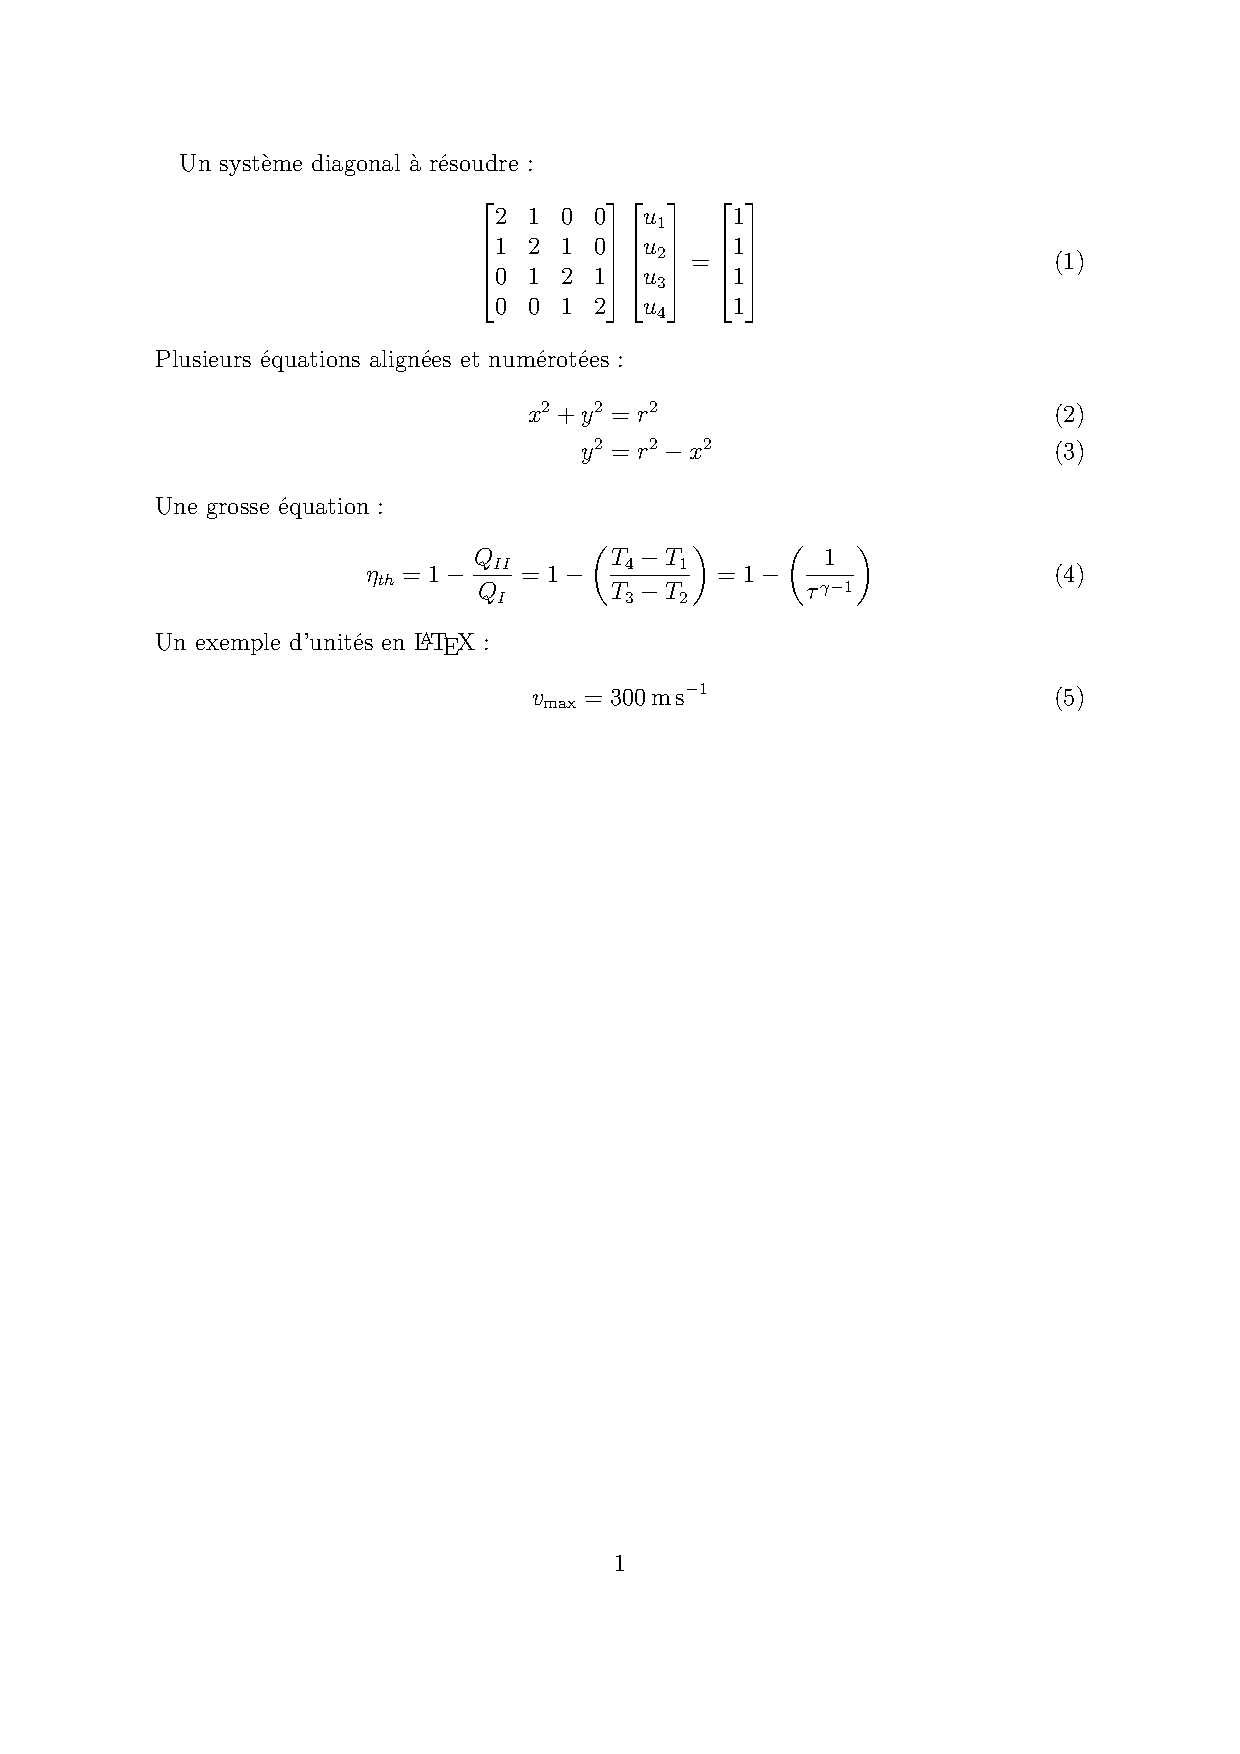
\includegraphics[width=0.8\textwidth,trim={2cm 16cm 2cm 2cm},clip]{exercices/3/build_latex/main.pdf}}
    \end{center}
\end{frame}

\begin{frame}[fragile]{Quatrième exercice (solution)}
\begin{center}
Lien Overleaf de la solution du quatrième exercice \url{https://www.overleaf.com/read/dqdzcnzsmnsh}
\end{center}
\end{frame}

\AtBeginSection[]{} %% stop TOC

\section{Ressources}
\subsection{conclusion}
\begin{frame}
  \frametitle{Pour aller plus loin}
  Chercher de l'information:
    \begin{itemize}
        \item \url{http://en.wikibooks.org/wiki/LaTeX}
        \item \url{http://bertrandmasson.free.fr/}
        \item \url{http://www.grappa.univ-lille3.fr/FAQ-LaTeX}
            \item \url{http://www.andy-roberts.net/writing/latex}
            \item \url{http://ctan.org/pkg/packagename} ou \lstinline[language=sh,morekeywords={texdoc}]{$ texdoc packagename}
        \item Google est ton ami !
            \item \url{https://www.overleaf.com/learn}
            \item La version de StackExchange spécialisée pour le \TeX:
  \url{https://tex.stackexchange.com}.
        \item Livres:
        \begin{itemize}
            \item \LaTeX HowTo par Sébastien Combéfis (EN/FR)
            \item Framabook \LaTeX
        \end{itemize}
    \end{itemize}
\end{frame}

\subsection{documentation supplémentaire}
\begin{frame}[fragile]
  \frametitle{Description}
  \begin{itemize}
    \item L'environnement \lstinline|description| permet de faire des définitions.
    \begin{lstlisting}[style=nonumbers]
\begin{description}
  \item[ODT] Open Document Text.
  \item[ODS] Open Document Spreadsheet.
  \item[ODP] Open Document Presentation.
\end{description}
    \end{lstlisting}
    \begin{description}
      \item[ODT] Open Document Text.
      \item[ODS] Open Document Spreadsheet.
      \item[ODP] Open Document Presentation.
    \end{description}
\end{itemize}
\end{frame}


\subsection{La chimie}
\begin{frame}[fragile]
  \centering
  \frametitle{La chimie}
  \begin{lstlisting}
\usepackage{chemfig}
...
\chemfig{*6(-=(-CH_2OH)-(-COOH)=-=)}
  \end{lstlisting}
  \begin{center}
    \chemfig{*6(-=(-CH_2OH)-(-COOH)=-=)}
  \end{center}
  \begin{lstlisting}
\usepackage[version=3]{mhchem}
...
  \[\ce{3H2O + 1/2H2O -> AgCl2- + H2_{(aq)}}\]
  \end{lstlisting}
  \[\ce{3H2O + 1/2H2O -> AgCl2- + H2_{(aq)}}\]
\end{frame}

\subsection{Les circuits}
\begin{frame}[fragile]
  \frametitle{Les circuits}
  \begin{lstlisting}
\usepackage{circuitikz}
...
\shorthandoff{:!} % Pour certaines versions de circuitikz
\begin{circuitikz}
  \draw (0,0) to [sI, v=$V_2$] (0,-3);
  \draw (6,-3) to[short, i = $I_2$] (0,-3);
  \draw (0,0) to [R = R, v = $V_R$] (3,0);
  \draw (3,0) to [L = L, v = $V_L$] (6,0);
  \draw (6,0) to [C = C, v = $V_C$] (6,-3);
\end{circuitikz}
\shorthandon{:!} % Pour certaines versions de circuitikz\end{lstlisting}
  \begin{center}
        \shorthandoff{:!}
    \begin{circuitikz}
      \draw (0,0) to [sI, v=$V_2$] (0,-3);
      \draw (6,-3) to[short, i = $I_2$] (0,-3);
      \draw (0,0) to [R = R, v = $V_R$] (3,0);
      \draw (3,0) to [L = L, v = $V_L$] (6,0);
      \draw (6,0) to [C = C, v = $V_C$] (6,-3);
    \end{circuitikz}
        \shorthandon{:!}
  \end{center}
\end{frame}

\subsection{Inclure du code}
\begin{frame}[fragile]
  \frametitle{Inclure du code}
  \begin{lstlisting}[mathescape=true]
\begin{lstlisting}
if a == b:
  return 0
else:
  return 1
\$\color{blue}{\texttt{end}}${lstlisting}\end{lstlisting}
donne
  \begin{lstlisting}[language=Python]
if a == b:
  return 0
else:
  return 1\end{lstlisting}

  Il y a aussi
  \begin{lstlisting}
\lstinputlisting[caption={...},label=...]{main.py}\end{lstlisting}
  et
  \begin{lstlisting}
\lstinline|if a == b|\end{lstlisting}
  qui donne \lstinline|if a == b|.
\end{frame}

\subsection{Dessiner en LaTeX avec Tikz}
\begin{frame}[fragile]
\frametitle{Dessiner en LaTeX avec Tikz}
    \begin{figure}[!ht] \centering
        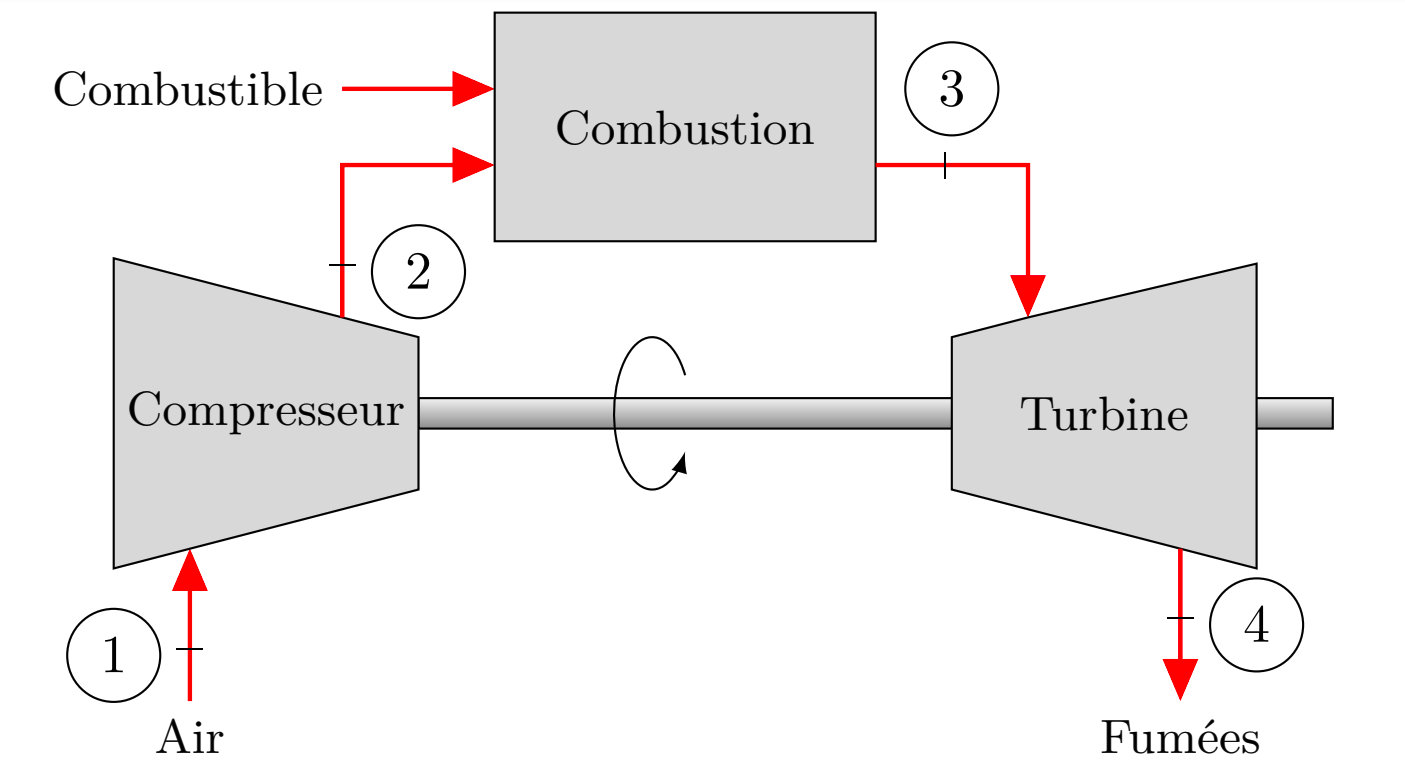
\includegraphics[width=0.8\textwidth]{img/turbine}
    \end{figure}
\end{frame}

\begin{frame}[fragile]{Les paragraphes avec \LaTeX{}}
  \framesubtitle{Alignement d'un paragraphe}
  \begin{itemize}
      \item Les environnements \lstinline|center|, \lstinline|flushright| et \lstinline|flushleft| permettent d'aligner un paragraphe.
    \begin{columns}
      \begin{column}{0.4\textwidth}
        \begin{lstlisting}[style=nonumbers]
Justifié; c'est le comportement par défaut de \LaTeX{}

\begin{center}
  Centré
\end{center}

\begin{flushright}
  Aligné à droite
\end{flushright}

\begin{flushleft}
  Aligné à gauche, mais pas justifié, comme vous pouvez le voir
\end{flushleft}
        \end{lstlisting}
      \end{column}
      \begin{column}{0.6\textwidth}
        \begin{mdframed}
          Justifié; c'est le comportement par défaut de \LaTeX{}

          \begin{center}
            Centré
          \end{center}

          \begin{flushright}
            Aligné à droite
          \end{flushright}

          \begin{flushleft}
            Aligné à gauche, mais pas justifié, comme vous pouvez le voir
          \end{flushleft}
        \end{mdframed}
      \end{column}
    \end{columns}
  \end{itemize}
\end{frame}

\begin{frame}[fragile]{Jouer avec la police}
\framesubtitle{Changer la taille de police}
  \begin{itemize}
      \item \lstinline|{\small text}| pour changer la taille du texte à l'intérieur
      \item \lstinline|\small| pour changer tout le texte jusqu'au prochain appel de \lstinline|\normalsize|
  \end{itemize}
  \begin{tabular}{ll}
  \lstinline|{\tiny polygenelubricants}| & {\tiny polygenelubricants} \\
  \lstinline|{\small polygenelubricants}| & {\small polygenelubricants} \\
  \lstinline|{\normalsize polygenelubricants}| & {\normalsize polygenelubricants} \\
  \lstinline|{\large polygenelubricants}| & {\large polygenelubricants} \\
  \lstinline|{\Large polygenelubricants}| & {\Large polygenelubricants} \\
  \lstinline|{\LARGE polygenelubricants}| & {\LARGE polygenelubricants} \\
  \lstinline|{\huge polygenelubricants}| & {\huge polygenelubricants} \\
  \lstinline|{\Huge polygenelubricants}| & {\Huge polygenelubricants} \\
  \end{tabular}
\end{frame}

\end{document}
